\documentclass[a4paper,11pt]{book}

\usepackage[utf8]{inputenc}
\usepackage[italian]{babel}
\usepackage[T1]{fontenc}
\usepackage[letterpaper,top=2cm,bottom=2cm,left=3cm,right=3cm,marginparwidth=1.75cm]{geometry}

% Useful packages
\usepackage{amsmath}
\usepackage{graphicx}
\usepackage[colorlinks=true, allcolors=blue]{hyperref}
\usepackage{listings}
\usepackage{amsthm}
\usepackage{amssymb}
\usepackage{pdfpages}

\usepackage{algorithm}
\usepackage{algpseudocode}

\theoremstyle{plain}
\newtheorem{theorem}{Teorema}[chapter]
\theoremstyle{plain}
\newtheorem{lemma}{Lemma}[chapter]
\theoremstyle{definition}
\newtheorem{definition}{Definizione}[chapter]

\usepackage{float}

\usepackage{listings}
\usepackage{color}

\definecolor{dkgreen}{rgb}{0,0.6,0}
\definecolor{gray}{rgb}{0.5,0.5,0.5}
\definecolor{mauve}{rgb}{0.58,0,0.82}

\lstset{
  language=xml,
  aboveskip=3mm,
  belowskip=3mm,
  showstringspaces=false,
  columns=flexible,
  basicstyle={\small\ttfamily},
  numbers=none,
  numberstyle=\tiny\color{gray},
  keywordstyle=\color{blue},
  commentstyle=\color{dkgreen},
  stringstyle=\color{mauve},
  breaklines=true,
  breakatwhitespace=true,
  tabsize=3
}

\title{Fondamenti di sicurezza e privacy}

\begin{document}
\maketitle

\thispagestyle{empty}

\tableofcontents

\thispagestyle{empty}
	
\cleardoublepage %%%% Add this one here!
\pagenumbering{arabic}

\setchapterpreamble[u]{\margintoc}
\chapter{Introduzione}
\labch{chapter1}

\paragraph*{Crittografia} Nasconde il contenuto del messaggio, ma non l'esistenza dello stesso.

\paragraph*{Stenografia} Nasconde l'esistenza del messaggio (es tecniche: inchiostro invisibile, codifico il messaggio nei bit meno significativi dell'immagine che non sono visibili a occhio nudo). Se qualcuno scopre la tecnica che nasconde il messaggio, allora tutti i messaggi che usano quella tecnica diventano visibili.

\paragraph*{Sistema sicuro} Non esiste un concetto assoluto di sicurezza, ma si può dire che un sistema è sicuro quando il costo necessario a romperlo è superiore al vantaggio economico che si otterrebbe/al danno che si produrrebbe.

\section{Breve storia della crittografia}

\paragraph*{Cifrario di Cesare} Uno dei primi metodi crittografici della storia è quello di \textbf{Cesare}. Si basa sullo shift dell'alfabeto di $n$ posizioni. La chiave corrisponde alla prima coppia di lettere dell'alfabeto originale e traslato (es: la chiave è AD, quindi per decifrare il messaggio devo prendere la lettera che corrisponde a 3 posizioni indietro rispetto a quella scritta nel messaggio cifrato -la lettera D cifrata corrisponderà alla lettera A-).
Si tratta di una cifratura facilmente attaccabile in quanto le \textbf{possibili chiavi} sono solo 26 (\textbf{tutti gli shift dell'alfabeto}).
Un attacco di questo genere (testo tutti i possibili shift) si chiama attacco di forza bruta: testo tutte le chiavi possibili finché trovo quella corretta.

\paragraph{Permutazione arbitraria dell'alfabeto} Un'evoluzione di questo metodo di cifratura è la \textbf{permutazione arbitraria}. Questo metodo si basa sulla permutazione totale dell'alfabeto, piuttosto che sul suo semplice shift. In questo caso la \textbf{chiave} è \textbf{alfabeto permutato}.
Le possibili chiavi sono $[26!]$ (50 anni fa non era facilmente attaccabile da attacchi di forza bruta a causa dei pc poco potenti). Questa cifratura è attaccabile con l'\textbf{analisi delle frequenze}\sidenote{L'analisi delle frequenze è lo studio della frequenza di utilizzo delle lettere o gruppi di lettere in un testo cifrato. Questo metodo si basa sul fatto che in ogni lingua la frequenza di uso di ogni lettera è piuttosto determinata; questo è vero in modo rigoroso solo per testi lunghi, ma spesso testi anche corti hanno frequenze non molto diverse da quelle previste. 
Tramite questa analisi è possibile inoltre determinare anche la lingua del messaggio, in quanto ogni lingua ha delle frequenze specifiche (tralasciando le lingue orientali).}. 
Nel caso si utilizzi un attacco a forza bruta (automatizzato dal pc), è possibile capire che se ho raggiunto il risultato corretto sempre tramite l'analisi delle frequenze. 

\paragraph{Counter all'analisi delle frequenze} Si propose di lavorare non più con una singola lettera, ma con coppie di lettere. In questo modo ad ogni lettera cifrata potevano corrispondere 2 lettere in chiaro. Uno degli approcci utilizzati è il seguente:

\begin{table}[H]
\centering
\begin{tabular}{|c|c|c|c|c|}
\hline
& & & & &
\hline 
& & & & &
\hline 
& & & & &
\hline 
& & & & &
\hline 
& & & & &
\hline 
\end{tabular}
\end{table}

\noindent Supponiamo di avere una tabella $5 \times 5$ che andrà a contenere una password che sarà la chiave. Usiamo la parola \textit{MONARCHY}. Nel caso la password contenga lettere ripetute, le ripetizioni vengono saltate, in modo che ogni lettera compaia una sola volta.

\begin{table}[H]
\centering
\begin{tabular}{|c|c|c|c|c|}
\hline
M & O & N & A & R &
\hline 
C & H & Y & & &
\hline 
& & & & &
\hline 
& & & & &
\hline 
& & & & &
\hline 
\end{tabular}
\end{table}

\noindent A questo punto procediamo inserendo le lettere dell'alfabeto mancanti, saltando ovviamente quelle già inserite. Consideriamo la lettera I uguale alla lettera J (ho 25 posti e le lettere sono 26).

\begin{table}[H]
\centering
\begin{tabular}{|c|c|c|c|c|}
\hline
M & O & N & A & R &
\hline 
C & H & Y & B & D &
\hline 
E & F & G & I/J & K &
\hline 
L & P & Q & S & T &
\hline 
U & V & W & X & Z &
\hline 
\end{tabular}
\end{table}

\noindent Possiamo procedere ora con la codifica, lavorando sulle coppie di lettere. Le regole da seguire sono:
\begin{itemize}
    \item Se la coppia di lettere da cifrare appartiene alla stessa riga nella tabella, si prenderà la lettera successiva nella riga, procedendo in maniera circolare.
    
    Esempio: Supponiamo di dover cifrare la coppia AR. Nella tabella AR appartiene alla stessa riga, quindi uso la regola sopra. La lettera A corrisponderà alla lettera R (mi sposto di una posizione), mentre la lettera R corrisponderà alla lettera M (essendo la fin della riga, la posizione successiva è l'inizio della riga stessa).
    
    Quindi:
    \begin{center}
        AR $\longrightarrow$ RM\\
        OA $\longrightarrow$ RN
    \end{center}
    
    \item Se la coppia appartiene alla stessa colonna, lavoro come nel primo caso, solo che qui mi sposto verso il basso sulla colonna.

    Esempio:
    \begin{center}
        MU $\longrightarrow$ CM
    \end{center}
    
    \item Se la coppia appartiene a righe e colonne diverse, la prima lettera si sposterà nella colonna della seconda e viceversa.
    
    Esempio:
    \begin{center}
        PB &$\longrightarrow$ SH\\
        EA &$\longrightarrow$ IM oppure JM
    \end{center}
    
\end{itemize}

\noindent Anche questo metodo è comunque attaccabile con l'analisi delle frequenze, in quanto, sebbene la codifica di una lettera dipende dall'altra della coppia (e quindi non valore più il caso di \textit{a lettera uguale corrisponde lettera uguale}), vale il caso in cui "a coppia uguale corrisponde coppia uguale" e anche le coppie di lettere di una lingua hanno le loro frequenze.

\paragraph{Cifrario di Vigenère} Il cifrario di Vigenère riprende l'idea del cifrario di Cesare: presa una chiave (es: \textit{key}), si ripete la chiave tante volte quanto è lungo il testo (eventualmente troncando l'ultima ripetizione), e si codifica la lettera con il corrispondete cifrario di Cesare. 

\noindent
K E Y K E Y K E Y K E Y \\
P R O V A D I T E S T O 
	
\noindent La prima lettera del cipher text sarà la lettera ottenuta dal cifrario di Cesare di chiave AP, la seconda con la chiave AR e così via.
Anche questo cifrario è semplice da attaccare, si parte dalla divisione del ciphertext in gruppi di lunghezza pari a quella della chiave, e si esegue l'analisi delle frequenze su ogni gruppo. Nel caso in cui non si conosca la lunghezza della chiave, si può semplicemente provare tutte le possibili lunghezze della chiave. Ovviamente sarà necessario un testo di dimensioni maggiori ai precedente per poter effettuare l'analisi. Se la password fosse lunga quanto il testo, l'analisi delle sequenze non sarebbe possibile.
	
\paragraph{One-time pad} Vediamo ora lo schema di Vigenère applicato ad un alfabeto binario. In questo caso il mio alfabeto si compone di soli due simboli: 0 e 1. Posso avere solo 4 casi di chiave-testo:
\begin{align*}
Key \rightarrow & 1 0 1 0 \\
Text \rightarrow & 0 1 0 1 \\
Cyph \rightarrow & 0 1 1 0 
\end{align*}

\noindent Praticamente applicare questo schema ad un alfabeto binario equivale ad applicare lo XOR tra testo in chiaro e chiave. Per riottenere il plaintext a partire dal cyphertext, mi basta riapplicare lo XOR tra chiave e cyphertext. Riassumendo:
\begin{align*}
    \text{Encryption } E(P, K) = P  \oplus K\\
    \text{Decryption } D(C, K) = C  \oplus K
\end{align*}

\noindent Se ho una chiave lunga quanto il testo e la chiave è scelta in modo casuale (ogni bit del testo è indipendente dalla chiave (viene scelto non conoscendo la chiave)):
\begin{itemize}
    \item La probabilità che il primo bit \textit{b} del cyphertext \textit{c} sia 0 è $\frac{1}{2}$ (lo stesso che sia uno);
    \item La probabilità che il primo bit del cyphertext sia 0 è
        \begin{align*}
            Pr[c = 0] &= Pr[b = 0 \land k = 0] + Pr[b = 1 \land k = 1]\\
                    &= P \cdot \frac{1}{2} + (1-P) \cdot \frac{1}{2}\\
                    &= \frac{1}{2} (P+1-P)\\
                    &= \frac{1}{2}
        \end{align*}
    \noindent Ovvero la probabilità che il cyphertext \textit{c} sia 0 è data dalla probabilità \textit{P} che il bit \textit{b} sia stato scelto con valore 0, moltiplicata la probabilità che il bit \textit{k} della chaive sia stato scelto a 0, sommata alla probabilità che il bit del plaintext \textit{b} sia stato scelto a 1, quindi \textit{P - 1}, moltiplicata la probabilità che \textit{k} sia 1.
\end{itemize}

\noindent Se scelgo la chiave in maniera casuale, a prescindere da come è stato scelto il plaintext, la distribuzione probabilistica sul cyphertext è quella uniforme. Quindi osservando il cyphertext vedo solo una sequenza casuale di bit, che non mi può dire nulla sul plaintext (ogni plaintext è equamente probabile dato il cyphertext). Questo sistema, detto \textbf{one-time pad}, è assolutamente sicuro.

\paragraph{Teorema di Shannon} Per avere un sistema crittografico sicuro, tale per cui a partire dal cyphertext non si può ricavare nulla del plaintext, allora la chiave deve essere tanto lunga quanto il plaintext. 

Secondo questo teorema, i sistemi usati oggi non sarebbero sicuri, in quanto usano chiavi con dimensione inferiore al messaggio scambiato. Per questo l'obiettivo è costruire sistemi dove, sebbene sia possibile ottenere informazioni dal cyphertext, questa operazione diventi troppo complessa (es: richiede molto tempo).
	
\section{Problemi di sicurezza non legati alla crittografia}
La sicurezza del dato non dipende solo dall'affidabilità del protocollo crittografico utilizzato. Rischi di sicurezza possono derivare, ad esempio, anche dalle implementazioni. 

Vediamo il caso dell'IBM 360. Il sistema utilizzava, per il controllo della password, il semplice controllo della stringa (si confronta la prima coppia di lettere e se uguali si passa alla seconda e così via) e memorizza la password in chiaro. Si riuscì a fare in modo che una parte della password inserita per il test finisse in una pagina di memoria, mentre il resto in una seconda pagina che finisce fuori dalla chache. Si faceva quindi partire il confronto e se il sistema ritornava un page fault\sidenote{Il page fault è un'eccezione generata quando un processo cerca di accedere a una pagina che è presente nel suo spazio di indirizzamento virtuale, ma che non è presente nella memoria fisica poiché mai stata caricata o perché precedentemente spostata su disco di archiviazione. Tipicamente, il sistema operativo tenta di risolvere il page fault caricando la pagina richiesta nella memoria virtuale oppure terminando il processo in caso di accesso illegale. Il componente hardware che rileva i page fault è il memory management unit, mentre quello software di gestione delle eccezioni è generalmente parte del sistema operativo (kernel). } allora la parte di password scritta nella prima pagina era corretta (se fosse stata errata il controllo si sarebbe fermato prima di raggiungere la seconda pagina, che essendo fuori dalla chache, dà page fault).

Un altro problema legato al controllo tramite confronto delle stringhe è che più lunga è la stringa, maggiore è il tempo necessario per terminare l'operazione. Si potrebbe quindi determinare la lunghezza della stringa contando i microsecondi necessari al completamento del controllo.
\chapter{Cyber Kill Chain}
\label{chapter2}

\paragraph{Threat intelligence} Analisi dei possibili attacchi informatici che possono colpire l'organizzazione. Determinare le fasi di un attacco e le sue tecniche permette di fare una scelta mirata sulle misure di protezione da adottare per prevenirlo o ridurne l'impatto. \\

\section{Fasi della cyber kill chain}
La cyber kill chain, in generale, descrive le fasi in cui può essere suddiviso un attacco:
\begin{enumerate}
    \item Reconnaissance: decidere e ottenere info sul target. La reconnaissance può essere:
\begin{itemize}
    \item Attiva: raccolgo info interagendo col target.
        \begin{itemize}
            \item nmap per creare una mappa della rete dell'obiettivo (porte disponibili, porte aperte, servizi associati); 
	        \item port scanning;
	          \item vulnerability scanner (es: nessus);
	        \item Linkedin per cercare ruoli specifici nell'organizzazione.
        \end{itemize}
    \item Passiva: raccolgo info senza interagire col soggetto.
	      \begin{itemize}
	          \item whois permette di raccogliere info su un dominio o specifico IP: quando è stato creato; data rilasco e scadenza certificato; chi è l'amministratore di sistema; contatto tecnico per rinnovo dominio;
	          \item Shodan: porte aperte; servizi accessibili; lista vulnerabilità;
	        \item Social media;
	        \item mantego.
	      \end{itemize}
\end{itemize}

	
\item Weaponization: trovare o creare l'attacco che exploita una vulnerabilità. Posso usare:
\begin{itemize}
    \item Metasploit per creare un attacco che sfrutta vulnerabilità. Fornisce codice già pronto per sfrittare vulnerabilità;
    \item Exploit DB;
    \item Vell Framework;
    \item Aircrack;
    \item SQL map;
    \item Cobal strike, tool legittimo a pagamento usato per penetration testing. Ha struttura modulare.
\end{itemize} 

\item Deliver: decido in che modo consegnare l'exploit. Posso sfruttare: siti web, social media, email, USB, ...

\item Exploitation: exploito una vulnerabilità. Posso usare:
\begin{itemize}
    \item  SQL injection;
    \item Buffer overflow;
    \item Malware;
    \item Javascript hijacking;
    \item User exploitation;
    \item Compromissione sito legittimo (inserimento script o sfruttamento vulnerabilità framewok usati nel sito).
\end{itemize}

\item Installation: mantengo persistente l'attacco all'interno dell'ambiente. Posso usare:
\begin{itemize}
    \item DDL hijacking;
\item Meterpreter;
\item Remote Access Trojan;
\item Registry chenges;
\item PowerShell commands.
\end{itemize}

\item Command and Control (C2): stabilisco un canale di C2 conl'attaccante per manipolare da remoto la vittima.

\item Actions and Objectives: eseguo azioni per reggiungere il goal originario. Posso:
\begin{itemize}
    \item Raccogliere credenziali utente;
\item Scalare privilegi;
\item Reconnaissance interna;
\item Movimento nell'ambiente;
\item Recccogliere dati;
\item Distruggere sistemi;
\item Riscrivere o corrompere dati;
\end{itemize}
\end{enumerate}

\section{Trickbot}
Torjan avanzato che si diffonde principalmente tramite campagne di spearphishing usando mail che contengono allegati malevoli o link che eseguono sw malevoli. Gli attacchi recenti usano mail di phishing.
\chapter{Panorama sui cyber threat}

\section{Overview 2022}
\begin{itemize}
    \item La maggior parte degli attacchi sono stati cybercrimini e sabotaggi/spionaggi;
    \item Tipologie principali attacchi: malware, phishing, attacchi web, sfruttamento vulnerabilità;
    \item Settori principalmente targetizzati: governo, salute, comunicazioni.
\end{itemize}

\section{Malware}
\paragraph{Ransomware as a service} catena che si compone di più attori:
\begin{itemize}
    \item Operatori: gang cybercriminali che dispongono delle capacità e risorse per creare e gestire ransomware e infrastrutture collegate;
    \item Affiliati: gang cybercriminali che affittano i ransomware dagli operatori;
    \item Access Brocker: gang cybercriminali che ricercano info o vulnerabilità su organizzazioni target;
\end{itemize}
Se l'attacco dell'affiliato ha succeso (infezione e riscatto), il guadagno viene condiviso con il relativo operatore.

\paragraph{Overview attacchi malware 2022}
\begin{itemize}
    \item Nell'ultimo anno il 66% delle aziende è stato colpito da un attacco ransomware;
    \item Costo medio del riscatto: \$900.000;
    \item Il 46\% delle aziende ha pagato il riscatto nonostante avesse dei backup;
    \item Il 61\% delle paganti è riuscita a ripristinare i dati;
    \item Solo il 4\% li ha ripristinati totalmente.
\end{itemize}

\section{Trend recenti negli attacchi malware}
\paragraph{Tecnica Double Extortion} Oltre alla richiesta di riscatto per ottenere la chiave di decifratura usata per cifrare i dati, la vittima viene minacciata con la diffusione di tali dati (preventivamente copiati dall'attaccante) nel caso di mancato pagamento (tecnica double extortion). 

\paragraph{Tecnica Triple Extortion} Funziona come la double extortion, solo che nel caso in cui l'azienda si rifiuti di pagare, gli attaccanti si rivolgono ai suoi clienti.

Una delle vittime di questo tipo di attacco è stata un'azienda finlandese di consulenza psichiatrica. Gli attaccanti hanno minaccaito i clienti di pubblicare le loro conversazioni private con gli psichiatri in caso di mancato pagamento del riscatto.

\paragraph{Intermittent Encryption} Tecnica che velocizza il tempo di infezione andando a cifrare solo alcuni byte/blocchi dei file. Tende ad evadere le analisi antimalware in quanto fa un uso limitato delle operazioni di lettura/scrittura su file.

\paragraph{Lockbit 3.0} Aggiornamento del malware Lockbit che introduce un programma di bug hunting con ricompensa.

\paragraph{BlackCat} Scritto in Rust, è uno dei primi ad implementare la crittografia intermittente. Offre features per pubblicare i dati e ricercare info sul target.

\paragraph{Attacco alla Ferrari} Attacco di supply chain o ransomware, non ancora verificato. Sono stati rubati 7GB di dati, contenenti progetti e manuali tecnici.

\paragraph{Altri attacchi} Sono stati attaccati il Gestore Servizi Energetici e l'università di Pisa.

\paragraph{Urnsif} Banking Trojan (malware che ruba credenziali dell'home banking o dati della carta di credito) che usa attacchi di phishing tramite mail, le quali contengono un documento office con macro che scarica Ursnif. Quando l'utente si collega all'home banking, il malware si attiva lanciando un alert di infezione che invita a scaricare una nuova app.

\paragraph{Attacco alla Colonial Pipeline} Effettuato ai danni della Colonial Pipeline, ha reso inutilizzabili i suoi sistemi di distribuzione del carburante. Questo attacco può essere inteso come un attacco alle strutture critiche (blocco trasporti, blocco attività, ...).

\paragraph{Nuove tecniche di evasione} Nel ransomware usato nell'attacco alla WastedLocker, creato in modo specifico per questo attacco (conosceva il nome dei file da cercare), è stata implementata una nuova tecnica per evitale la rilevazione da parte del sistema. In generale, molti sistemi anti-malware vanno a ricercare nei programmi il richiamo a specifiche api di Windows (es: apertura file, lettura, cifratura). Per evitare questo problema, il malware ha utilizzato il Windows Cache Manager. Invece di cifrare i dati direttamente su disco, e venire quindi rilevato, ha usato questo manager per caricarli in memoria e cifrarli qui, per poi risalvarli su disco.

\paragraph{Botnet} Usati per attacchi DDoS e per distribuire altri malware. I principali sono Emotet e Trickbot. Emotet nasce inizialmente nel 2016 come Financial Trojan, per poi evolversi come mezzo per scaricare altri malware. L'anno scorso, grazie ad un'operazione dell'Europol, ha perso terreno. A novembre è però risorto.

\paragraph{Malware cellulari} Tra i più famosi c'è Pegasus, spyware usato da molti governi per controllare personaggi di interesse. MasterFred, altro malware mobile, invece va a costruire sopra le interfacce legittime di pagamento di varie app (es: Netflix) delle interfacce fasulle, sfruttando le impostazioni di accessibilità di Android.
 
\paragraph{FluBot} Si tratta di un malware Android/IOS, che ha come obiettivo i dati relativi alle carte di credito, diffusosi molto tramite sms contente i link infetti. Generalmente il messaggio si spacciava come proveniente da Un'azienda di trasporti (es: DHL) che richiedeva di installare l'app allegata per facilitare/velocizzare la consegna.

\section{Attacchi comuni}
\paragraph{Attacchi di phishing (ultimi 6 mesi)} Targetizzati INPS e BPER Group (banca).

\paragraph{Smiching} Attacchi di ingegneria sociale tramite sms.

\paragraph{Vshing} Voice phishing -> nella mail di phishing non metto un link ma un numero di telefono da contattare (es: contattare servizio clienti per tentato accesso all'account paypal).

\paragraph{EvilProxy} Permette di superare le autenticazioni a due fattori eseguendo un attacco di \textit{man in the middle}.

\paragraph{Compromissione di siti legittimi} Hijacking di siti legittimi;

\paragraph{Uso di HTTPS} Ora anche i siti malevoli potrebbero avere una connessione HTTPS, quindi la presenza di certificato non assicuro la legittimità del sito. 

\section{Attacchi cloud}
\paragraph{Vulnerabilità OMIGOD} I ricercatori di sicurezza hanno rivelato i dettagli di quattro vulnerabilità, note collettivamente come OMIGOD, che interessano lo strumento Open Management Infrastructure (OMI) di Microsoft. Sostengono che un utente malintenzionato remoto non autenticato può sfruttare alcune o tutte queste vulnerabilità per ottenere l'accesso amministrativo all'ambiente virtuale Linux in esecuzione sul servizio di cloud computing Azure di Microsoft.

\paragraph{ChaosDB} ChaosDB è una vulnerabilità critica nel servizio di database Azure Cosmos DB di Microsoft. Un utente malintenzionato potrebbe sfruttarlo per ottenere l'accesso in lettura/scrittura alle informazioni del database di altri utenti, nonché all'infrastruttura di hosting di Azure sottostante.

\section{Attacchi a dispositivi IoT}

La maggior parte dei dispositivi IoT è vulnerabile ad attacchi di media/alta gravità. Questo è dovuto a quattro fattori principali:
\begin{enumerate}
    \item Il traffico dati non è criptato;
    \item Molto spesso gli utenti non cambiano password e continuano ad usare quella di default;
    \item I sistemi operativi usati (principalmente relativi al controllo industriale) sono spesso non aggiornati;
    \item In generale hanno bassa memoria, capacità computazionale, spazio per salvare e potenza
\end{enumerate}

\paragraph{BadAlloc} Una ricerca di Microsoft ha scoperto che molti dei dispositivi che usano sistemi embedded o real time scritti in C sono facile preda di attacchi di Buffer Overflow (C è noto per le vulnerabilità legate alla gestione della memoria). Il problema è dovuto alle librerie C di allocazione dinamica della memoria (heap): se alla malloc si passa un integer che causa Integer Overflow (numero negativo o troppo grande), l'attaccante può sovrascrivere la memoria allocata dalla malloc ed eseguire codice malevolo.

\paragraph{Classe di vulnerabilità Ripple20} è stato scoperto che questa libreria, implementata in molti dispositivi, sono presenti 19 vulnerabilità, di cui 4 molto gravi.

\paragraph{Telecamere di videosorveglianza} Molto spesso nei sistemi di videosorveglianza non sono implementati sistemi di autenticazione o, se lo sono, utilizzano sistemi deboli (es: password).

Sul sito \href{https://www.shodan.io/}{https://www.shodan.io/} è possibile ricercare tutti i dispositivi IoT collegati alla rete e ricavarne informazioni. Può essere usato per studiare attacchi mirati.

\paragraph{*Malware Mirai} Da varie ricerche si è scoperta che telecamere re e stampanti sono i dispositivi IoT meno sicuri. Mirai è un malware progettato per operare su dispositivi connessi a Internet, specialmente dispositivi IoT, rendendoli parte di una botnet che può essere usata per attacchi informatici su larga scala. Scansiona continuamente la rete alla ricerca di dispositivi accessibili protetti da password di default o molto comuni (es: abc123, admin123, 1234, password, ...).

\paragraph{Vulnerabilità nei dispositivi healthcare} Il settore della healthcare è tra quelli più vulnerabili ad attacchi informatici. Tra i dispositivi più a rischio troviamo i sistemi di imaging (es: radiografie) e di monitoraggio dei pazienti. Ad esempio, Medtronic è stata costretta a ritirare dal mercato diverse pompe di insulina a causa di una vulnerabilità che consentiva di modificare i valori della pompa (rischio coma glicemico).


\chapter{Social engineering} 
L'ingegneria sociale è la manipolazione psicologica delle persone per far si che eseguano azioni o divulghino informazioni personali. Sfrutta le vulnerabilità insite nelle persone.

Secondo Kevin Mitnick, uno degli hacker più famosi al mondo, anche se l'organizzazione investe pesantemente in sistemi di sicurezza, se l'attaccante riesce a fare quello che vuole anche a una sola persona, tutto l'investimento fatto è inutile.

Alcuni cyber criminali che usano l'ingegneria sociale sono:
\begin{itemize}
    \item Hacker: attacchi DDoS, ransomware, attacchi finanziari;
    \item Identity thieves: usano info che identificano la persona per i loro obiettivi (e poi possono rivenderle/pubblicarle online);
    \item Scam artists: eseguono azieni fraudolente o ingannevoli per frodare altri (es: lotteria scam su facebook).
\end{itemize}

\paragraph{Attacco alla banca del Bangladesh} Nel 2016 la banca del Bangladesh è stata vittima di una delle più grandi rapine informatiche. L'attacco è iniziato nel 2015, quando gli attaccanti sono riusciti ad installare un malware utilizzando un file malevolo spacciato per curriculum per una delle posizioni aperte nella banca. Lo scopo del malware era di eseguire una serie di trasferimenti verso una società no-profit estera. L'attacco è stato sventato dalla Federeal Reserve, dalla quale passano i trasferimenti internazionali, che si è accora dell'attacco grazie ad un errore di spelling nel nome dell'associazione.

\paragraph{Attacco a Macron} Caso di Identity Steal. Due francesi sono riusciti ad accedere alla mail di Macron, dalla quale hanno inviato mail che descrivevano i 10 motivi per cui non votare Macron.

\paragraph{Lotteria su Facebook} La persona viene contattata tramite Facebook informandola della vincita ad una lotteria e che l'assegno le verrà recapitato a casa. Alla consegna, alla vittima viene chiesto un pagamento per ricevere l'assegno.

\section{Ciclo di vita dell'attacco}
\begin{enumerate}
    \item Selezione del target;
    \item Reconnaissance;
    \item Raccolta delle info: posso cercare nella spazzatura della vittima ("dumpster diving" -> cerco bollette, stampe conto corrente, post-it con login e password, ...) o la osservo standone in prossimità ("shoulder surfing");
    \item Orchestrazione dell'attacco;
    \item Esecuzione dell'attacco: sfrutto le info e le relazioni per spingere la vittima a compiere le azioni che voglio;
    \item Impatto dell'attacco: raggiungo il mio obiettivo (es: installazione malware, eliminazione tracce attacco sulla macchina della vittima, ...).
\end{enumerate}

Possibili modi per ottenere informazioni: osservare alla spalle il target (es: mentre la persona sta lavorando al pc), cercare nella spazzatura del target.

\paragraph{Esempio di attacco}
\begin{itemize}
    \item  Obiettivo: ottenere dalla vittima le info necessarie ad eseguire un trasferimento di denaro;
    \item Selezione del target, reconnaissance, raccolte info: ad esempio verifico online se il target è stato vittima di attacchi di data breach;
    \item Attacck orchestration: ad esempio contatto la vittima tramite mail+telefono o sms+telefono;
    \item Esecuzione dell'attacco: 
	\begin{enumerate}
	    \item  Creo lo stage per l'attacco, creando ad esempio un sito web di phishing che simula il sito web di autenticazione della banca della vittima;
	    \item Creo un app malevola da far installare alla vittima, la quale mi girerà i codici ricevuti necessaria a superare l'autenticazione a più fattori;
	    \item Invio una mail alla vittima con il link alla pagina web;
	    \item  Contatto al vittima per telefono e la convinco a installare l'app. Per incrementare le possibilità di successo, posso camuffare il numero di telefono usando tecniche di spoofing facendo comparire il numero di telefono della banca;
	    \item  Se tutto ha successo, ottengo accesso all'home banking della vittima. 
	\end{enumerate}
    \item Impatto dell'attacco: Elimino ogni traccia dell'attacco (es: l'app si rimuove terminato il suo lavoro).
\end{itemize}

\section{Tipi di attacchi}
\begin{itemize}
    \item Phishing: condotto generalmente via mail, cerca di attaccare più persone possibili. Generalmente l'attaccante si finge una persona di alto rango o richiede che un'azione vengo svolta entro un breve limite di tempo;
    \item Spear phishing: mira ad una persona particolare;
    \item Whaling: mira a persone con elevate responsabilità nell'organizzazione;
    \item Viral hoaxe: mira a divulgare info false e quindi influenzare l'opinione delle persone. Sfrutta la curiosità delle persone (diffuso nei social, dove il post chiede di aprire il link per avere più info sull'argomento);
    \item Vhishing: usa chiamate telefoniche;
    \item Impersonation e tailgating: fatti di persona;
    \item SMiShing attacco tramite SMS.
\end{itemize}

\paragraph{Impersonation} Solitamente mi fingo qualcuno con autorità, qualcuno con seniority o un ente governativo.

\paragraph{Vishing} Un esempio di attacco è stato quello del falso servizio clienti di Apple. L'attaccante chiamava la vittima fingendosi il servizio clienti di Apple dicendo che c'era un problema con l'account Appl. Quando la vittima richiamava per risolvere, l'attaccante chiedeva i dati di accesso dell'account.

\paragraph{Tailgating} Sfrutta l'indole delle persone ad aiutare gli altri (es: mi fingo un dipendente della banca che ha dimenticato il tesserino di accesso l'accesso, mi accodo ad un dipendente e chiedo se posso passare con lui; mi fingo un dipendente dell'azienda che ha versato il caffè sopra dei documenti e chiedo di ristamparli. I documenti sono in una chiavetta che installa poi il malware).

\section{Attacchi di phishing}
Il phishing è il tentativo di acquisire informazioni sensitive come username, password e dettagli di carte di credito (e a volte, indirettamente, denaro), spesso con scopi malevoli, spacciandosi per un'entità di fiducia in comunicazioni elettroniche.
\\

\noindent Dati:
\begin{itemize}
    \item L'88\% delle organizzazione mondiali è stato vittima di un attacco di spear phishing nel 2019;
    \item Il 95\% degli attacchi alle reti aziendali deriva da un attacco andato a buon fine di spear phishing;
    \item Il 22\% delle violazioni dei dati nel 2019 ha riguardato il phishing;
    \item Il 97\% degli utenti non è in grrado di riconoscere mail di phishing sofisticate;
    \item Il 30\% delle mail di phishing vengono aperte;
    \item Nel 12\% di queste, il link viene clickato;
    \item Il 15\% delle vittime viene targetizzato da almeno un altro attacco nello stesso anno.
\end{itemize}

\paragraph{Attacchi che sfruttano la pandemia} Durante la pandemia Google ha bloccato milioni di mail che proponevano un raccolta fondi per finanziare la ricerca di un vaccino.

\paragraph{Possibili indicatori che la mail è di phishing}:
\begin{itemize}
    \item Non mi stavo aspettando quella mail con quel contenuto;
    \item Errori grammaticali nel testo o nell'oggetto;
    \item Indirizzo del mittente o del CC strano;
    \item Link effettivo (che vedo muovendoci sopra il mouse) diverso da quello scritto;
    \item Assenza della grafica classica di quel tipo di mail;
\end{itemize}

\noindent \textbf{Attenzione}: l'anteprima della mail dal client solitamente mostra solo il nome del mittente e non anche il suo indirizzo; molto spesso i link presenti nella mail di phishing usano servizi di URL shortening.\\

\noindent \textbf{PhishTank}: sito web che, dato il link ad una pagina web, questo rientri tra la lista dei siti conosciuti di phishing.

\section{Attacchi di spearphishing}
Un attacco di spearphishing è un attacco di phishing lanciato specificamente contro un'organizzazione o un utente target, spesso adattato alla vittima rappresentando informazioni uniche per loro al fine di creare autenticità.

\section{Tattiche di influenza}
Posso "usare":
\begin{itemize}
    \item Autorità: assumo una posizione di autorità rispetto alla vittima (manager, ceo, direttore risorse umane, ente governativo);
    \item Scarsità: una risorsa limitatamente disponibile spinge la vittima ad agire con velocità;
    \item Commitment: le persona agiscono in maniera consistente. Se una persona ha svolto un'azione in passato, è probabile che la rifaccia. Quindi posso prima chiedere alla vittima informazioni poco sensitive per poi passare a quelle che  i interessano (es: prima chiedo il nome del cane e poi la risposta alle domande per recuperare il codice di un account);
    \item Liking: le persone tendono ad eseguire un'azione se viene chiesta da persone che conoscono;
    \item Reciprocità: se alla vittima viene offerto qualcosa è più probabile che esegua l'azione (es: per ricevere il premio è necessario aprire il link);
    \item Social proof: la vittima tende a svolgere l'azione se altre persone l'hanno già svolta.
\end{itemize}

\section{Come un'organizzazione può fermare gli attacchi di phishing}
In figura \ref{fig:my_label3} è riportato come un'organizzazione può fermare gli attacchi di phishing.
\begin{figure}
    \centering
    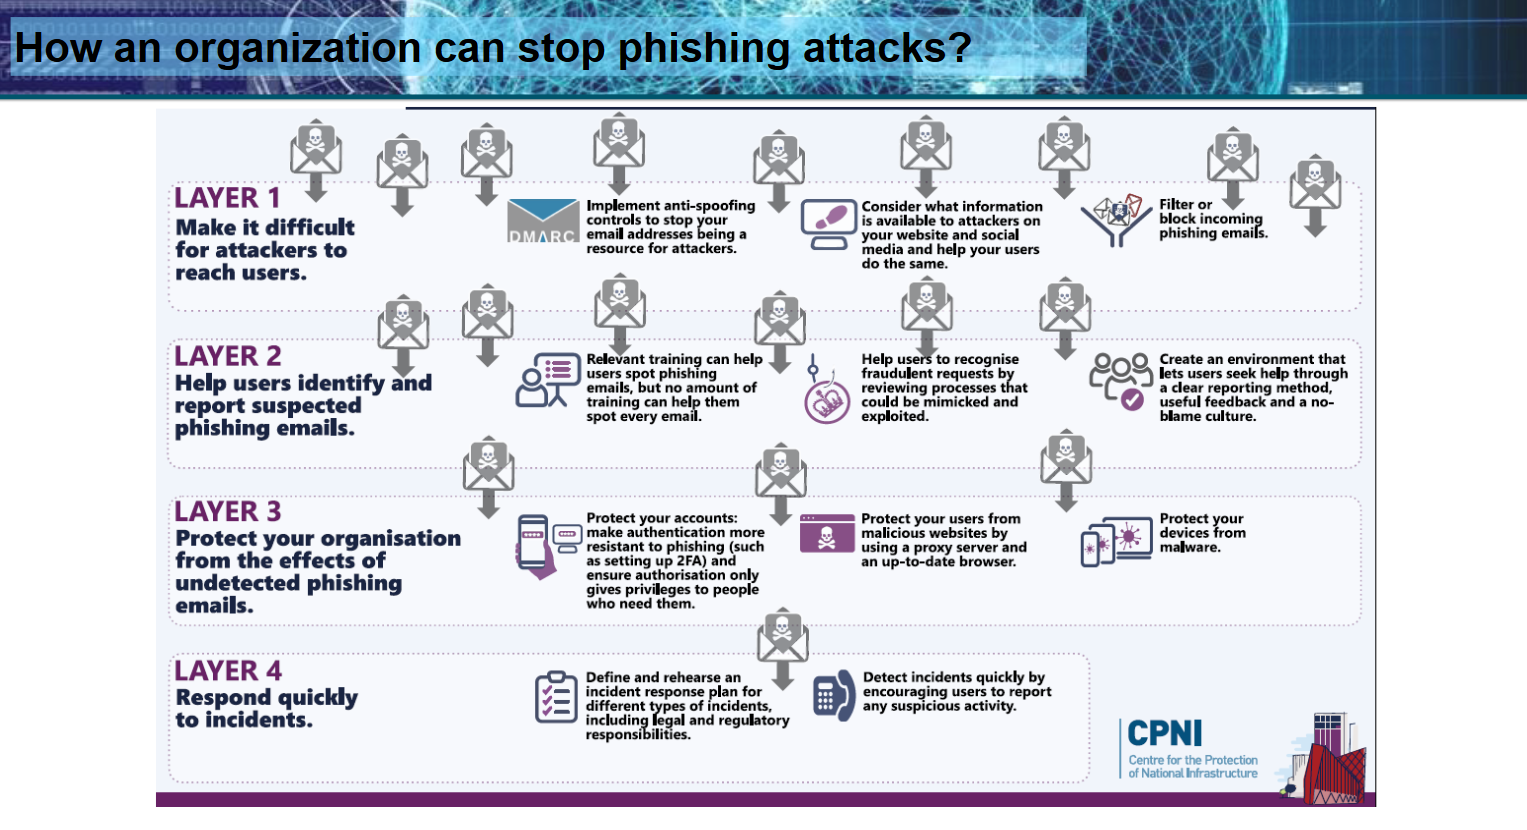
\includegraphics[width=1\textwidth]{images/5.png}
    \caption{Come fermare gli attacchi di phishing}
    \label{fig:my_label3}
\end{figure}
\chapter{Malware}

Un malware (contrazione di malicious + software) è un software malevolo che compie azioni che mirano a compromettere la riservatezza, disponibilità o l'integrità dei dati o dei sistemi infettati.

I sistemi possono venire infettati tramite:
\begin{itemize}
    \item Accesso diretto al sistema con dischi/chiavette USB infetti;
    \item Attacchi di ingegneria sociale;
    \item Campagne di phishing;
    \item Visitando siti malevoli.
\end{itemize}

\section{Tipi di malware}
\paragraph{Virus} Modifica/altera/compromette file o sw presenti sulla macchina della vittima. Ha la capacità di riprodursi, infettando le altre macchine presenti nella stessa rete. Richiede però l'azione umana per essere eseguito (link email, sito malevolo, apertura documenti malevolo). Questo tipo di malware è facilmente identificabile dagli antivirus, in quanto i virus hanno una specifica signature riconoscibile. I tipi di virus principali sono tre:
\begin{enumerate}
    \item Macro virus, codificati come una serie di comandi inseriti in una macro all'interno del file malevolo (pdf, doc, ...). Non c'è quindi un eseguibile vero e proprio, ma si compone di comandi scritti in un linguaggio di scripting (es: VBA, powershell, ...);
	\item Virus polimorfici, che cambiano il loro comportamento a seconda dell'OS dove vengono eseguiti o a seconda dei sw presenti nella macchina;
	\item Companion virus, i più insidiosi in quanto si mascherano come sw legittimo (aggiornamento sw o sw comunemente presenti nelle macchine windows).
\end{enumerate}

\paragraph{Worm} Simile al virus, ha l'obiettivo di permettere all'attaccante di ottenere il controllo della macchina. Questo viene solitamente fatto installando backdoor. Ottenuto il controllo, l'attaccante può rubare i dati presenti. Si può replicare nelle altre macchine presenti nella rete. Non necessitano di azione umana in quanto sfruttano vulnerabilità presenti nella macchina (OS, protocolli, ...).

\paragraph{Trojans} Tra le tipologie più diffuse. Nato come sw malevolo che accede ad info sensitive sulla macchina della vittima (credenziali, info finanziarie, ...), è diventato nel tempo uno strumento usato per mantenere il controllo della macchina della vittima (installando una backdoor). Una volta ottenuto il controllo, solitamente vengono sfruttati per installare altri malware;
\paragraph{Rootkit} Solitamente installato nel kernel (che si interfaccia tra le componenti sw e hw della macchina), monitora tutte le chiamate di funzioni a libreria effettuate dal sw in esecuzione permettendo di mascherare la presenza di altri malware nella macchina della vittima andando ad intercettare le chiamate a Windows API effettuate dagli altri malware. Offre anche funzionalità di accesso come amministratore/root alla macchina.

Esistono tre categorie principali di Rootkit:
\begin{enumerate}
	\item Quelli a livello applicativo;
	\item Quelli a livello del kernel (kernel rootkit);
	\item Quelli  installati nel master boot record.
\end{enumerate}

I primi, che vengono mascherati come sw legittimo, sono facili da rimuovere (dagli antivirus), i restanti sono più difficili in quanto vanno a compromettere l'OS. Per eliminarli solitamente è necessario reinstallare il sistema.

\paragraph{Dropper/downloader} Il dropper è un malware che contiene al suo interno il vero malware da infettare. Tipicamente prende la forma di macro incluse all'interno di allegati malevoli. Quando il documento viene aperto, la macro viene eseguita e il malware estratto. 

Il downloader, invece, non include il malware al suo interno, va a scaricarlo da un sito malevolo.

\paragraph{Keylogger} Malware che viene solitamente installato dal altri malware. Cattura tutti i caratteri digitati su tastiera, li salva in un file nascosto e periodicamente manda una copia del file all'attaccante (mail o command \& control).

\paragraph{Bot} Pone la macchina infetta sotto il controllo dell'attaccante. Solitamente vengono posto sotto il controllo di un pc chiamato Bot Master, che invia comandi agli zombi. Tipicamente questo viene utilizzato per creare reti di bot (botnet) per effettuare attacchi DDoS. Uno scenario tipico è quello dove il bot master impartisce il comando ping verso uno specifico target, fintanto che l'obiettivo non è più in grado di rispondere.

\paragraph{Cripto Miner} Utilizza le macchine infette per minare criptovalute e trasferirle nel wallet dell'attaccante. Molti di questi usano software di mining open source.

\paragraph{Ransomware} Cifra i file nella macchine della vittima. La chiave di decifratura è fornita a fronte di un pagamento.

\section{Prevenzione e riduzione dei danni}
\paragraph{Come posso prevenire la  la ricezione di malware}
\begin{itemize}
    \item  Uso un sw di antispam e che vada ad analizzare il contenuto delle mail (link e file);
    \item Uso security gatewway che vanno ad ispezionare il contenuto di alcuni dei protocolli di rete, come quello smtp, per cercare se sono presenti malware noti;
    \item Blocco l'accesso a siti potenzialmente malevoli a livello del browser con specifici plug-in, che si appoggiano ad una lista di url in cui è sicuro navigare;
\end{itemize}

\paragraph{Come posso prevenire la diffusione del malware alle altre macchine della rete}
\begin{itemize}
    \item Mantengo l'OS aggiornato per impedire al malware di usare vulnerabilità ora patchate;
    \item Prevengo l'accesso alle credenziale dell'amministratore o di specifici utenti, utilizzando sistemi di autenticazione MFA (es: oltre a utente e password richiedo una One Time Password che arriva tramite sms);
    \item Limito i privilegi degli utenti che hanno accesso alle macchine (solitamente gli amministratori di sistema concedono più permessi del necessario), per limitare le azioni che il malware può effettuare;
    \item Faccio usare all'amministratore due account differenti: il primo per gestire la parte social (email, comunicazioni, ...), e che è quindi più soggetto a campagne di phishing, e il secondo, con utente e password diversi dal primo, per gestire la rete.
\end{itemize}

\paragraph{Educazione dei dipendenti}
\begin{itemize}
    \item Educo sulle tecniche di ingegneria sociale usare per diffondere i malware;
    \item Educo sulle tipologie di malware esistenti;
    \item Educo sui rischi che comporta un'infezione per l'organizzazione e su come limitare i danni;
    \item L'educazione deve essere fatta in maniera continua, per stare al passo con l'evoluzione tecnologica.
\end{itemize}

\paragraph{Backup regolari}
\begin{itemize}
    \item Mantengo più copie dei file e sw utilizzando diversi meccanismi (es: cloud) e/o dispositivi (es: disco esterno alla rete aziendale). I backup devono essere effettuati offline e tenuti in posizioni separate dalla rete/sistema dell'azienda. Per sicurezza effettuo più copie;
    \item Mi assicuro che i dispositivi contenenti il backup non devono essere lasciati collegati perennemente alla rete;
    \item Mi assicuro che i backup sono connessi solo a dispositivi puliti prima di iniziare il ripristino. Per sicurezza, scansiono i backup alla ricerca di malware prima di iniziare il ripristino.
    \item Mantengo aggiornati i programmi di backup.
\end{itemize}

\paragraph{Ripristino in seguito ad attacco malware}
\begin{itemize}
    \item  Sconnetto tutti i dispositivi infetti dalla rete;
    \item Spengo il Wi-Fi e disabilito ogni connessione importante della rete (es: switch);
    \item Formatto i dispositivi in modo sicuro e reinstallo l'OS;
    \item Scansiono il backup alla ricerca di malware;
    \item Ricollego il dispositivo ripristinato ad una rete pulita ed eseguo le installazioni/aggiornamenti necessari;
    \item Installo, aggiorno e avvio un antivirus;
    \item Riconnetto il dispositivo alla rete dove era precedentemente collegato;
    \item Controllo il traffico di rete e scansiono alla ricerce di infezioni rimanenti.
\end{itemize}

\section{Ransomware}

Esistono molte famiglie di ransomware, che differiscono per le tecniche che implementano nelle varie fasi della cyber kill chain di un attacco ransomware. Possono colpire tutti i sistemi operativi.\\

\paragraph{Tipi}
\begin{itemize}
    \item Encryption malware: cifrano i dati;
    \item Locker: bloccano l'interfaccio utente con cui l'utente ha accesso all'OS e mostrano una schermata in cui si richiede un riscatto in cambio dello sblocco;
    \item Master Boot Record ransomware: cifra il master boot record o lo modifica in modo che l'os non sia più caricabile;
    \item Wiper: cancella i file presenti sulla macchina, senza possibilità che la vittima li recuperi.
\end{itemize}

\paragraph{Componenti principali di un ransomware}
\begin{itemize}
    \item Componente trojan: ha il compito di far arrivare il ransomware sulla macchia della vittima. Può implementare tre tipi di consegna:
	\begin{enumerate}
        \item Tramite email di phishing con allegato malevolo;
        \item Tramite Exploit Kit che sfrutta vulnerabilità dell'OS o del sw;
        \item Tramite la compromissione di siti legittimi;
	\end{enumerate}
    \item Componente di cifratura/decifratura: generalmente vengono usati due tipi di cifratura:
    	\begin{enumerate}
    	    \item Simmetrica per cifrare i dati della vittima (la cifratura simmetrica è veloce);
    	    \item A chiave pubblica (asimmetrica) per cifrare la chiave simmetrica. Una volta cifrata viene inviata all'attaccante, che possiede la chiave privata.
    	\end{enumerate}
    \item Routin di estrazione della chiave: estrae la chiave utilizzata per cifrare i dati e la invia all'attaccante (solitamente la chiave viene generata nella macchina infetta);
    \item Interfaccia con l'utente: presenta le istruzioni per pagare il riscatto.
\end{itemize}

\paragraph{Fasi della cifratura}
\begin{itemize}
    \item Genero la chiave simmetrica -> può essere generata al momento nelle macchine, inviata dall'attaccante tramite il command and control server o codificata nel codice del ransomware (soluzione usata agli inizi);
    \item Cifro i dati con la chiave simmetrica;
    \item Cifro la chiave simmetrica con la chiave pubblica e la invio all'attaccante;
    \item Cancello la chiave simmetrica dalla macchina della vittima.
\end{itemize}

\noindent I primi ransomware usavano tecniche di cifratura primitive o deboli:
\begin{itemize}
    \item Analizzando il codice del malware è possibile risalire alla chiave codificata nel codice;
    \item La cifratura con XOR e RC4 sono deboli ad attacchi di forza bruta.
\end{itemize}


\subsection{Killer switch}
Si tratta condizioni implementate dagli sviluppatori del malware per stoppare il loro funzionamento (possono essere state lasciate all'interno per errore).

\paragraph{Kill Switch per WannaCry} Il funzionamento di questo ransomware era legato alla registrazione di uno specifico domain name. Il ransomware andava inizialmente a controllare se il dominio era attivo, tramite DNS request, e, se riceveva l'indirizzo IP come risposta, andava ad effettuare una richiesta HTTP al dominio. Se riceveva anche qui risposta, bloccava la sua esecuzione. Registrando il dominio è stato possibile bloccare globalmente il malware.

\paragraph{Killer Switch per Bad Rabbit} L'obiettivo di questo malware era distruggere il Master Boot Record della macchina. Si è scoperto che se il malware non riusciva a scrivere su disco il file \textit{C:$\backslash$Windows$\backslash$infpub.bat}, la cifratura veniva stoppata. Questo killer switch non ne bloccava però la propagazione sulla rete.

\subsection{Cyber kill chain di un attacco ransomware}
\begin{enumerate}
    \item La vittima riceve una mail di phishing contenente un link ad un sito malevolo. La vittima visita il sito;
    \item Il server web, che sta hostando un exploit kit, analizza la macchina della vittima alla ricerca di vulnerabilità;
    \item Sfruttando le vulnerabilità trovate, il ransomware viene consegnato alla macchina ed si esegue;
    \item L'eseguibile elimina le eventualy shadow copy presenti nel pc (introdotte da windows, sono copie di backup di file) e si propaga nel file system;
    \item Il ransomware ricerca file con specifiche estensioni e li cifra;
    \item Il ransomware contatta il C\&C per inviare all'attaccante la chiave di cifratura e info sulla macchina;
    \item Il ramnsomware riceve info sul pagamento dal C\&C;
    \item Il ransomware mostra le info sul pagamento all'utente:
    	\begin{itemize}
    	    \item Se l'utente paga, il ransomware contatta il C\&C per riottenere la chiave per decifrare la chiave usata per cifrare. Non è detta che la chiave venga fornita;
           \item Se l'utente non paga entro il limite di tempo la chiave viene cancellata.
    	\end{itemize}
\end{enumerate}

\paragraph{Fase di weaponization}
\begin{itemize}
    \item Ransomware basato su script-> inserisco in un allegato una macro che carica in memoria lo script malevolo. Difficile da individuare da parte degli antivirus;
    \item Diversificazione del payload: nascondo il payload malevolo in file con differenti formati (es: odt, PDF, SVG, dll, ...). I client di posta bloccano mail contenenti eseguibili, quindi inserisco i ransomware all'interno di altri file;
    \item Diversifico i pattern di accesso ai file: il classico pattern apertura file-cifratura-salvataggio file è facilmente individuabile dagli antivirus. Per evitare di essere scoperto posso modificare l'estensione del file prima di salvarlo oppure posso rimuovere i file eliminando le info associate ai file, che sono salvate nella MFT (Master File Table), presente in tutti i file system NTFS (in questo modo posso rimuovere l'accesso al file senza doverlo cifrare).
\end{itemize}

\paragraph{Fase di evasione}
Tecniche per rendere più difficile il riconoscimento e/o l'analisi:
\begin{itemize}
    \item Time-based evasion techniques: per rallentare l'analisi o la scoperta del malware posso fare in modo che cifri i file solo in risposta a determinati eventi nel pc oppure inserire dei periodi di sleep nella fase di cifratura;
    \item Data evasion techniques: eliminano le tracce del malware dal pc della vittima (es: file di config, log, ...). Per evitare l'analisi posso usare anche le tecniche di anti-dump: generalmente per analizzare in un malware si aspetta che venga caricato tutto in memoria e poi, con sw specifici, viene scaricato. Tento di impedire questa tecnica per bloccare l'analisi.
    \item Code evasion techniques: prevedono tecniche di anti-debugging, anti-disassembling (es: cifro il ransomware, aggiungo offuscamento impacchetto il malware per evitare il disassemblaggio per la generazione del codice macchina) e anti-sandboxing (es: blocco o modifico il comportamento del malware se eseguito su una macchina virtuale -> controllo il mac address per capire se sono in un macchina virtuale in quanto vmware e virtualbox usano pattern specifici) per evitare l'analisi 
    \item Network evasion techniques: cifra, anonimizzano il traffico (usando reti anonime) o cambiano l'indirizzo IP del C\&C (domain shadowing);
\end{itemize}

\paragraph{Fase di delivery}
\begin{itemize}
    \item Phishing;
    \item Spearphishing;
    \item Malvertisement: la vittima clicca su un link pubblicitario e viene rediretta ad un sito infetto che hosta il ransomware o verso un exploit kit che cerca vulnerabilità nel sistema;
    \item Sistemi di distribuzione del traffico: redirigono il traffico di un sito web legittimo verso uno malevolo che hosta un malware drive-by-download.
\end{itemize}

\paragraph{Fase di exploitation}
\begin{itemize}
    \item Exploit kit;
    \item Vulnerabilità del target (vulnerabilità zero-days e vulnerabilità trovate durante la ricognizione).
\end{itemize}

\paragraph{Fase di installazione}
\begin{itemize}
    \item Rendere i file della vittima inaccessibili (cifro i file, li zippo in un archivio protetto da chiave, cifro il master boot record, distruggo i backup);
    \item Diffusione attraverso la rete.
\end{itemize}

\paragraph{Fase di command and control (C2)}
Durante la fase di command and control si ha la comunicazione tra il C2 e il ransomware. La comunicazione può avvenire in due momenti dell'infezione: 
\begin{itemize}
    \item Prima del processo di cifrature, se la chiave non viene generata sulla macchina della vittima, ma sul C2;
    \item Dopo che è terminato il processo di cifratura, per comunicare all'attaccante il chiave di cifratura e ricevere dal C2 le info di pagamento.
    Parte fondamentale di questa parte è la comunicazione col C2: 
    \item Nei ransomware più \textit{naive} (== ingenui), gli IP dei C2 sono solitamente presenti come una lista nel codice dei ransomware -> posso risalire e blacklistare questi indirizzi /domini;
    \item Nei ransomware più "furbi", viene implementato un Domain General Algorithm, che prevede che ransomware e C2 si mettano d'accordo sull'algoritmo da usare per generare il nome dei domini associati ai C2. In questo modo il nome viene generato dinamicamente ogni volta che il C2 viene contattato, rendendo quindi impossibile blacklistare il dominio. 
    \item Si può anche utilizzare un bot di un botnet esistente come C2.
\end{itemize}

\paragraph{Fase di actions and objectives}
Il ransomware raggiunge il suo obiettivo. Nel caso di un encryption ransomware l'obiettivo è di portare le vittime a pagare il riscatto. Questo può essere fatto:
\begin{itemize}
    \item Dando direttamente l'IBAN/paypal account alla vittima (strategia molto ingenua);
    \item Richiedendo pagamenti in criptovalute;
    \item Creando portali dedicati per supportare l'operazione di pagamento;
\end{itemize}

In alcuni ransomware sono presenti siti ospitati sulla rete Thor (garantisce l'anonimia) che fungono da servizio clienti del pagamento del riscatto.

\section{Wanna Cry}
Sfrutta una vulnerabilità del protocollo SMB usato da Windows per condividere file e accedere a dispositivi come le stampanti. Questa vulnerabilità consentiva all'attaccante di eseguire codice in remoto sulla macchina Per sfruttare questa vulnerabilità è stato usato l'EternaBlue exploit kit.  

Una volta arrivato su una macchina infetta che implementa il protocollo SMB, utilizza EternalBlue per installare una backdoor sulle macchine che sono collegate alla macchina infettata e che utilizzano anch'esse il protocollo SMB per condividere file con la macchina. Tramite la backdoor, l'attaccate va ad installare una copia di Wanna Cry e lo esegue.  Un altro modo utilizzabile per arrivare sulle macchie è sfruttare tecniche di ingegneria sociale per far pluggare delle chiavette USB infette col ransomware nelle macchine delle vittime. L'esecuzione avviene sfruttando la funzionalità di autorun: basta modificare il file di autorun della chiavetta per fare eseguire in automatico il ransomware.

Un altro modo ancora consiste nel sfruttare la funzione di file share, usati nelle organizzazioni per effettuare il backup dei dati. Di solito è presente un server, usato per la condivisione dei file, a cui si connettono tutte le macchine dell'organizzazione. Il pc infetto carica sul server dedicato al file sharing una copia del ransomware e, quando le altre macchine si connetteranno, andranno a scaricare la copia caricata. Una variante di questa tecnica consiste nel non scaricare il file stesso, ma creare dei link al file. Quando viene creato un link (es: link su desktop ad un file per renderlo più facilmente accessibile), viene creato un file LNK. All'interno di questi file è possibile includere dei comandi, che vengono eseguiti quando si clicca sul file LNK. Così basta inserire il comando per eseguire il ransomware sulla macchina dove è stato copiato il file LNK. 

\section{Prevenzione specifica per gli attacchi ransomware}
Molti consigli sono gli stessi visti per gli attacchi di ingegneria sociale. 
\chapter{Cyber War e attacchi ad infrastrutture critiche}
La cyber war è una guerra condotta tramite reti e computer. Di solito coinvolge due paesi, dove l'attaccante impiega un gruppo di hacker per sabotare strutture critiche dell'altro paese tramite cyber weapons (solitamente malware molto specializzati). 

Un gruppo di hacker nord koreano che effettua un attacco DDoS a uno dei maggiori provider telefonici americani NON è un attacco di cyber war. Un attacco di cyber war dovrebbe avere un impatto sulla vita sociale/economica/politica della nazione colpita. 
Un gruppo di hacker cinese che attacca una stazione elettrica americana può essere considerato un attacco di cyber war, in quanto l'obiettivo è una struttura critica e l'assenza della corrente elettrica ha un grande impatto sulla vita dei cittadini.

\paragraph{Infrastrutture critiche} Infrastrutture, sistemi, siti, informazioni, persone, reti o processi necessari al funzionamento e vita di una nazione. Comprendono anche quelle organizzazioni, persone e siti che non sono critici al mantenimento dei servizi essenziali, ma la cui protezione è necessaria a causa del grande pericolo che possono provocare al pubblico (es: nucleare civile, siti chimici).

\paragraph{Elenco strutture critiche} Trasporti pubblici, rete elettrica, comunicazione difesa, servizi di emergenza, finanza, salute, centrali nucleari, ...

\paragraph{Principali pericoli} Poiché queste infrastrutture forniscono servizi vitali per la vita di tutti i giorni, sono interessato a garantirne la disponibilità, l'integrità e la safety (es: attacco che modifica la velocità della turbine per farla esplodere -> può ferire gli operatori vicini). In figura \ref{fig:my_label4} sono riportati alcuni dei principali attacchi conosciuti.

\begin{figure}
    \centering
    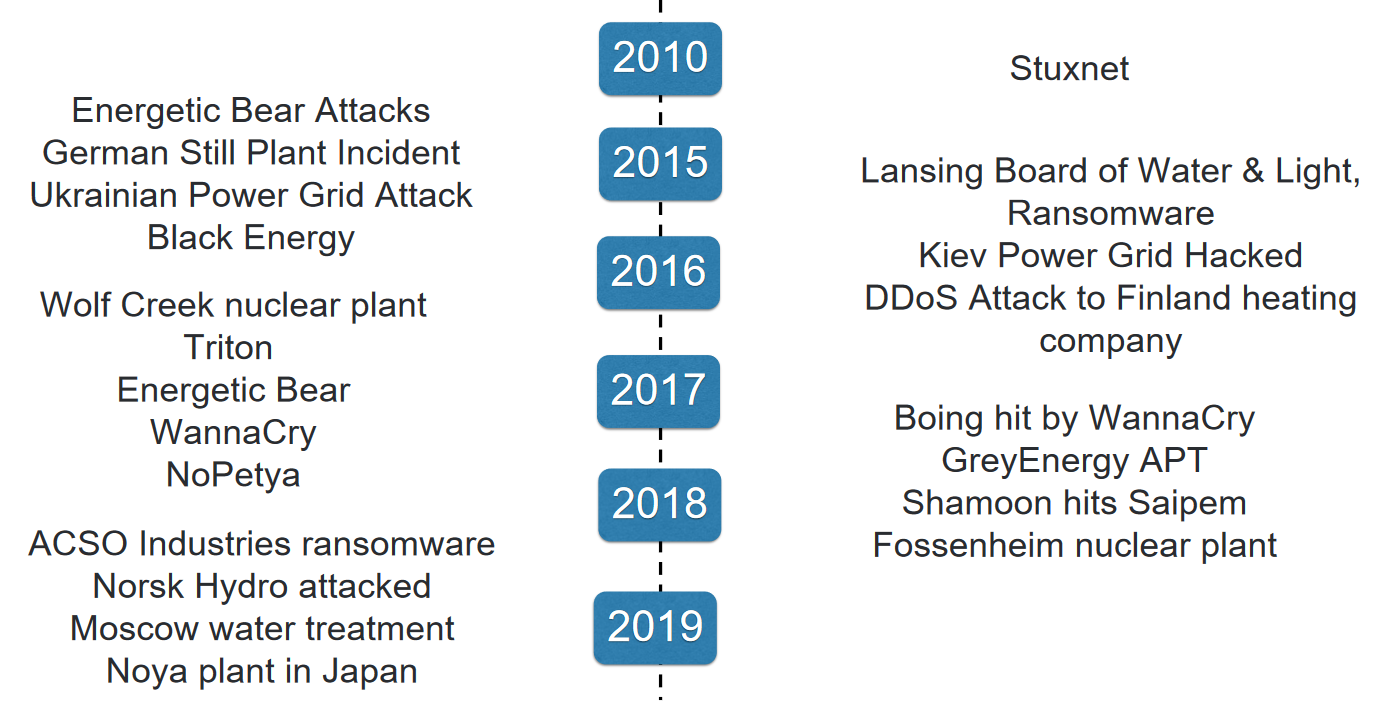
\includegraphics[width=1\textwidth]{images/6.png}
    \caption{Principali attacchi alle infrastrutture critiche}
    \label{fig:my_label4}
\end{figure}

\section{Sistemi di controllo industriale}

La maggior parte delle strutture critiche sono controllate e monitorate da sistemi di controllo industriale (ICS), che garantiscono la sefaty e la disponibilità. 

\paragraph{Componenti degli ICS} Ho uno o più processi da monitorare (produrre una macchina, sollevare la sbarra del parcheggio, produrre energia elettrica), implementati su macchine a cui sono associati sensori, che ne catturano i dati sul funzionamento. I dati cono verificati da un controllore. Il sistema di controllo industriale implementa due tipi di controllori: 
\begin{itemize}
    \item Uno più vicino alle macchine, che implementa il processo di controllo industriale. Prende il nome di Program Logic Controller (PLC) - quello che posso vedere con \href{https://shodan.io}{https://shodan.io};
    \item Uno più distribuito, chiamato SCADA, che controlla tutti i dispositivi coinvolte nel processo industriale.
\end{itemize}

Il controllore comunica con la Human Machine Interface (HMI), che è l'interfaccia usata dall'operatore. L'operatore invia dei comando al controllore, che li inoltra agli attuatori.

\paragraph{Sistemi SCADA} Tra i sistemi più diffusi, è un sistema distribuito consiste di un server che comunica con più stazioni (es: quelle per la distribuzione dell'energia elettrica locali di ogni città) e ne raccoglie i dati. I dati raccolti vengono salvati in un Data Historian ed utilizzabili dagli operatori in caso di necessità. Gli operatori possono anche, tramite le Engineering Workstation, inviare comandi alle diverse stazioni. Un esempio di dispositivo che posso trovare nelle stazioni locali sono gli interruttori per trasmettere l'energia elettrica 

Questi sistemi presentano diverse vulnerabilità. 

La più importante è legata al fatto che  inizialmente questi sistemi erano chiusi, quindi non connessi alla rete. Ora sempre di più utilizzano connessioni internet normali per funzionare. Questo li espone logicamente ad una serie di attacchi.

Molto spesso, inoltre, per garantire la disponibilità dei servizi, il ciclo di vita del macchianario viene estessa molto (circa 10-20 anni). Quindi molti dei sistemi in uso utilizzano sw obsoleti non più supportati dal venditore.

Un'altra problematica è legata all'accesso a questi dispositivi. Molti dei sistemi di autenticazione utilizzano l'autenticazione con password, che viene spesso lasciata a quella di default.

Spesso non vengono mantenuti log delle attività svolte dai vari sipositivi, rendendo quindi difficile ricostruire gli attacchi subiti.

\section{Cyber kill chain per attacchi ICS}

Per gli attacchi agli ICS è stata sviluppata una cyber kill chain specifica. Secondo la ricerca svolta, questa si compone di due fasi:
\begin{itemize}
    \item La prima ha l'obiettivo di ottenere accesso alla rete dell'ICS, e segue le stesse fasi viste nella cyber kill chain classica.
    \item La seconda fase è quella in cui avviene l'attacco vero e proprio. che si divide in: sviluppo, test, consegna, installazione ed esecuzione dell'attacco all'ICS.
\end{itemize}

Supponiamo che il mio obiettivo sia modificare il sw che gira sul PLC che controlla gli interruttori che attivano/bloccano il trasferimento della corrente elettrica. Per fare ciò sviluppo un malware specifico, che posso testare sul medesimo PLC presente nella stazione che ho acquistato a priori sul mercato (il mio attacco è molto specifico, quindi devo effettuare dei test prima di metterlo in pratica). La delivery del malware la posso fare tramite campagne di phishing oppure sfruttando una chiavetta USB portata all'interno da un insider. 
	
\subsection{Esempi di attacchi reali}

\paragraph{Stuxnet} Prima cyber weapon. Può essere considerato ad oggi il malware più sofisticato mai realizzato. Sviluppato dai servizi di sicurezza americani e dell'intelligence israeliana per sabotare lo sviluppo nucleare iraniano. la cyber kill chain di Stuxnet è riportata in figura \ref{fig:my_label5}.

\begin{figure}
    \centering
    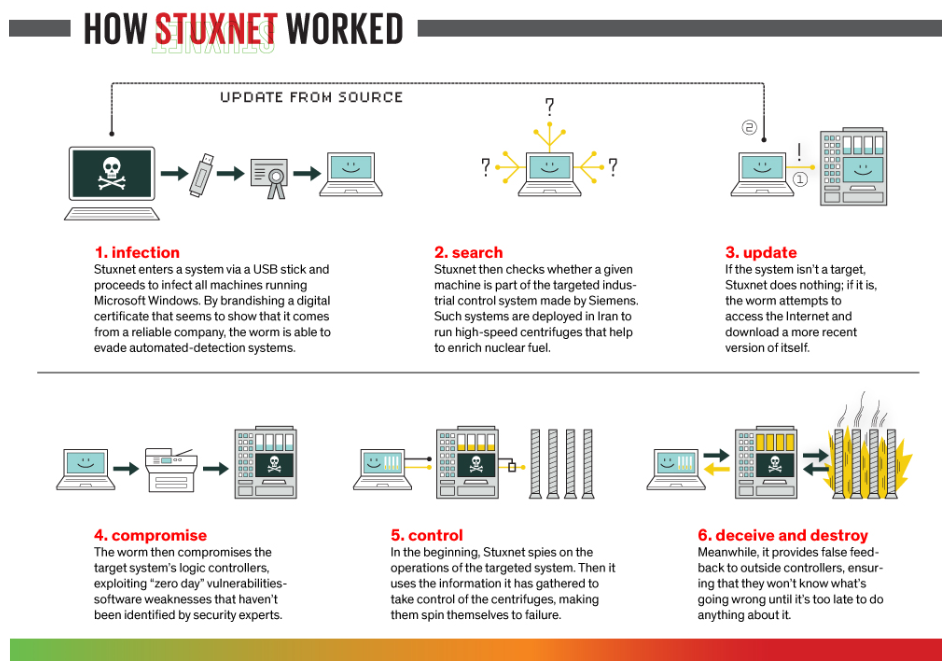
\includegraphics[width=1\textwidth]{images/7.png}
    \caption{Cyber kill chain di Stuxnet}
    \label{fig:my_label5}
\end{figure}

\noindent Stuxnet utilizza due tecniche di propagazione:
\begin{enumerate}
    \item Propagazione tramite network:
	\begin{itemize}
	    \item Infettando le macchie WinCC sfruttando hardcoded passwed (psw salvate in chiaro);
    	\item Propagandosi sfruttando la vulnerabilità zero-day MS10-061 Print;
    	\item Propagandosi sfruttando la vulnerabilità  MS08-067 del Windows Server Service;
	\end{itemize}
    \item Propagazione tramite dispositivi rimovibili, tramite:
    \begin{itemize}
        \item Vulnerabilità LNK (CVE-2010-2568);
    	\item Autoorun.inf.
    \end{itemize}
\end{enumerate}

\noindent Quando veniva infettata una chiavetta USB, venivano creati nella chiavetta tre file: un collevamento a Shortcul.lnk e due file temporanei.Quando la chiavetta veniva inserta, veniva eseguito lo shortcut, che andava a caricare il primo file tmp, che a sua volta caricava il secondo, che conteneva effettivamente il malware. 
	
Nella prima parte del file Autorun.inf c'era la copia di stuxnet. Questo è visibile dal fatto che ogni eseguibile Windows inizia con i caratteri $MZ$. 
Quando la chiavetta veniva pluggata, l'autorun rimandava all'esecuzione del programma che conteneva.
	
La parte di Commando e Control permetteva di staricare versioni aggiornate del malware, ma sembra che questa feature non sia mai stata usata.
	
Stuxnet andava a infettare pc che eseguivano il programma Step7, che consentiva di leggere e scrivere i programmi eseguiti dal PLC, e sostituiva una  libreria legittima che permetteva di modificare il codice eseguito dal PLC, e quindi lanciare comandi, con una versione malevola.
La libreria permetteva di modificare la velocità dei rotori delle turbine (per farle surriscaldare) o modificare la pressione del gas inserito (causando un aumento critico).

\paragraph{Attacchi del gruppo Sandworm} Gruppo affiliato al governo russo. I membri sono autori di diversi attacchi ad infrastrutture critiche di diversi paesi a partire dal 2015, come:
\begin{itemize}
    \item Attacco alla rete elettrica ucraina;
    \item Campagna di Spearphishing contro i membri del partito del presidente Macron (2017);
    \item Infezioni col ransomware NotPetya (2017);
    \item Attacchi contro le olimpiadi invernali (2017);
    \item Rallentamento delle investigazioni sulla morte della spia Novick (2018);
    \item Campagne contro infrastrutture critiche e siti governativi della Georgia.
\end{itemize}

\noindent Il primo attacco è stato effettuato il 23 dicembre 2015 in una stazione elettrica in Ucraina, che ha causato il blackout in una regione dei dintorni della capitale Kiev per qualche ora. Questo è stato il primo attacco ad una struttura critica.
L'obiettivo dell'attacco erano le stazioni di distribuzione dell'energia elettrica. 

Generalmente, un sistema di distribuzione si compone di una centrale che produce l'energia e la trasferisce alle stazioni di trasmissione, che ne abbassano il voltaggio e la trasferiscono agli utenti finali. Sandworm aveva compromesso gli interruttori che consentivano al trasmissione agli utenti, impedendola.

L'attacco si è strutturato come segue:
\begin{itemize}
    \item Tramite una campagna di spearphishing, ai danni del personale amministrativo e IT, gli attaccanti installano BlackEnergy 3 sulle macchine delle vittime (tamite macro malevola);
    \item BlackEnergy 3 stabilisce una connessione C2 con gli attaccante;
    \item Viene installato KillDisk nell'ambiente per rendere le macchine Windows/workstation inutilizzabili eliminando o modificando il master boot record;
    \item Viene lanciato un attacco DoS telefonico ai call center della compagna elettrica per impedire ai client di segnalare i problemi.
\end{itemize}
 \\
 
\noindent  Il 17 dicembre 2016, Sandworm ha attaccato la trasmissione dell'energia elettrica nella capitale Kiev. L'attacco è stato simile a quello precedente: mesi prima è stata effettuata nuovamente una campagna di spearphishing per ottenere accesso alla rete. Questa volta però il malware usato era Industroyer. Si tratta di un malware di complessità simile a stuxnet, ed è il secondo malware mai creato per sabotare un sistema industriale. Il suo obiettivo era quello di rendere inutilizzabili i remote terminal unit che controllavano gli interruttori per la trasmissione dell'energia elettrica. Si componeva di moduli che implementavano i quattro possibili protocolli di comunicazione che la work station degli operatori utilizzava per inviare i comandi ai remote terminal unit delle stazioni di trasmissione. Implementava anche un attacco DDoS contro i protection relay, i meccanismi che permettevano di richiudere gli interruttori in caso si verificasse una situazione anomala. 

 Industroyer aveva struttura modulare, con una main backdoor che permetteva l'accesso alla rete dell'azienda. Questa installava inoltre un'altra backdoor, utilizzata nel caso la prima fosse eliminata e scaricava due tool, uno per rubare le credenziali delle work station e l'altro per effettuare l'attacco DDoS. Il cuore del malware è rappresentato dal launcher, che implementava ed eseguiva i quattro payload che implementavano i quattro possibili protocolli di comunicazione. 
\\

\noindent NotPetya era un ransomware che colpì inizialmente l'Ucraina, per poi diffondersi in tutto il mondo. 
In Ucraina venne diffuso come update del software di contabilità fiscale M.E.Doc (molto usato nel paese): Sandworm era stata in grado di intercettare il traffico degli aggiornamenti di questo sw e ridirigerlo in un server situato in Francia, da cui installavano il malware. Una volta installato iniziava a cifrare i dati delle macchine infette. Presentava però delle stranezze rispetto ad un normale ransomware:
\begin{itemize}
    \item Usava lo stesso indirizzo bitcoin per il riscatto in ogni infezione;
    \item Richiedeva di riceve per mail la conferma del pagamento;
    \item Se la macchina aveva più dischi, generava una chiave per ciascuno;
    \item Inviava al server una stringa casuale come ID della vittima (per identificare la chiave usata);
    \item Non prevedeva una funzionalità per riceve la chiave di decifratura.
\end{itemize}



	
	
	
	

\chapter{Autenticazione dell'utente}
Il processo di autenticazione è uno dei primi metodi utilizzabili per proteggersi da attacchi informatici. Consiste nel verificare l'identità dell'utente, ovvero che sia chi dice di essere. 
Questo è importante per:
\begin{itemize}
    \item Garantire la proprietà di authentication -> se ho l'identità di un utente verificata, gli posso associare i permessi per lui previsti all'interno del sistema;
    \item Garantire la proprietà di accountability -> posso determinare chi ha effettuato determinate azioni all'interno del sistema (mantengo log sull'utente).
\end{itemize}

Ci sono tre modi principali per verificare l'identità di un utente, che possono essere usati singolarmente o in combinazione:
\begin{itemize}
    \item Tramite un segreto che l'utente possiede;
    \item Tramite qualcosa che l'utente possiede;
    \item Tramite qualcosa che l'utente è.
\end{itemize}

\paragraph{Sistemi token-based} Si utilizza un token generato da un'app, un dispositivo (OTP), una smart card o un barcode per autenticarsi. 
I dispositivi OTP solitamente implementano un algoritmo di hashing per generare la OTP, che prende in input un segreto memorizzato sul device/app. Il codice generato ha solitamente una validità limitata (30-60 secondi) e può essere usato in un'unica sessione di autenticazione. L'algoritmo più usato è il Time Based One Time Password Generation Algorithm, che prende in input un clock interno sincronizzato con quello del server di autenticazione per generare la OTP (utilizzo quindi il tempo).

L'altra tecnica token-based usata è quella che prevede l'uso delle smart card (carta con un piccolo processore), dove vengono memorizzati i certificati della chiave pubblica e della chiave privata rilasciati agli utenti. Per poter utilizzare la smartcard per autenticarsi è necessario utilizzare un lettore per collegarla la pc. Il processo di autenticazione segue un protocollo di challenge and response: 
\begin{itemize}
    \item Prima di tutto l'utente sblocca la carta con il pin associato;
    \item Il lettore genera un valore casuale che invia alla smart card;
    \item La card genera a sua volta un valore casuale e lo combina con quello del lettore. Firma il risultato con la chaive privata;
    \item Il lettore verifica la validità della firma con la corrispondente chiave pubblica.
\end{itemize}

\noindent Problemi: posso perdere/mi viene rubato il sistema che mi genera il token, rendendomi impossibile accedere al sistema. 

\paragraph{Autenticazione con sistemi biometrici} Come per le smart card, è necessario uno scanner della caratteristica biometrica che l'utente usa per autenticarsi. 
Le caratteristiche utilizzabili per autenticarsi devono essere:
\begin{itemize}
    \item Universali -> comuni a tutti gli individui;
    \item Distintive -> ogni persona dovrebbe avere differenze notabili in quella caratteristica;
    \item Permanenza -> la caratteristica non dovrebbe cambiare notevolmente nel tempo;
    \item Collezionabili -> la caratteristica dovrebbe essere effettivamente determinabile e quantificabile.
\end{itemize}

\noindent La caratteristica viene quantificata tramite lo scanner e salvata. Al momento dell'autenticazione, il sistema confronterà il dato precedentemente salvato con quello quantificato al momento: se la differenza è limitata, l'utente viene autenticato.

\noindent Esempi: firma, impronta digitale, retina, voce, volto, ...

\noindent Problemi: gli algoritmi usati possono generare falsi positivi (autorizzo un utente che non sarbbe autorizzato) e falsi negativi (non autorizzo un utente legittimo); a seconda della caratteristica scelta, un attaccante potrebbe facilmente rubarla (es: impronta digitale); l'utente potrebbe non voler farsi scannerizzare una determinata caratteristica. 

\section{Autenticazione con password}
Si tratta di sistemi semplici e poco costosi da implementare, ma molto vulnerabili ad attacchi, principalmente in quanto richiedono agli utenti uno sforzo cognitivo superiore a quello che sono in grado di effettuare. 

Uno dei problemi è che gli utenti utilizzano le stesse password sia in ambito domestico e lavorativo.

\subsection{Attacchi alle password}
Esistono diversi attacchi che permettono agli attaccanti di ottenere le password delle vittime:
\begin{itemize}
    \item Offline attacks: hanno l'obiettivo di accedere al **password file** salvato sul server di autenticazione in cui sono contenute tutte le password degli utenti;
    \item Online attacks: possono essere attivi o passivi. Richiedono che gli attaccanti interagiscano con l'obiettivo dell'attacco (es: servizio di cui voglio ottenere la password per accedere, account sul pc dell'organizzazione). Negli attacchi attivi, l'attaccante prova diverse password per trovare quella corretta, mentre in quelli passivi utilizza altri metodi, come l'intercettazione del traffico dell'utente;
    \item Non technical attacks: utilizzano tecniche di ingegneria sociale per ottenere le credenziali.
\end{itemize}

\noindent Tra le tecniche di attacco ci sono:
\begin{itemize}
    \item Attacchi di brute force;
    \item Attacchi con key logger;
    \item Attacchi con mail di phishing;
\end{itemize}

\subsection{Attacchi offline}
Dove sono memorizzate le password?
\begin{itemize}
    \item In Windows il password file è accessibile in due modi: 
    	\begin{itemize}
    	    \item In C:$\backslash$Windows$\backslash$System32$\backslash$config nel file SAM;
    	    \item Nei registri di Windows sotto HKEY\_LOCAL\_MACHINE -> SAM -> SAM. 
    	\end{itemize}
     \noindent Solitamente l'accesso al file è garantito solo ad account amministratore o system.
    \item In Linux ci sono due file usati per salvare la password:
    	\begin{itemize}
    	    \item $\backslash$etc$\backslash$passwd contiene gli user di tutti gli utenti collegati alla macchina;
        	\item $\backslash$etc$\backslash$shadow contiene gli hash delle password memorizzate nel password file.
    	\end{itemize}
\end{itemize}

\noindent Generalmente un password file memorizza quattro parametri per le password (separati da $:$):
\begin{itemize}
    \item Utente;
    \item SID;
    \item Due Hash.
\end{itemize}

![[]]

\noindent Salva quindi il nome dell'utente, un SID associato a tale nome e due hash della password, create tramite due algoritmi differenti:
\begin{itemize}
    \item LM: usato da sistemi windows fino alla versione XP. Crea hash a 128 bit ma utilizza un character set set di 142 caratteri e accetta password si max 14 caratteri. Divide la password in due sottostringhe di 7 caratteri e non è case sensitive (genera lo stesso hash se le due password sono uguali ma una con caratteri maiuscoli e una minuscoli);
    \item NTLM: introdotto successivamente e più sicuro. Crea hash a 128 bit ma utilizza tutti i caratteri ASCII e accetta password di max 256 caratteri. Non divide la password ed è case sensitive.
\end{itemize}

\noindent Per motivi di compatibilità, nelle versioni più recenti di Windows, sono presenti entrambi gli hash. 

\paragraph{Algorimo LM}
\begin{itemize}
    \item Memorizza password di max 14 caratteri;
    \item Converte tutti i caratteri a MAIUSCOLI;
    \item Filla gli spazi vuoti della passwword fino a raggiungere 14 caratteri;
    \item Divide la password in due sottostringhe di 7 caratteri;
    \item Cifra separatamente le due sottostringhe;
    \item Combina i due risultati.
\end{itemize}

 ![[]]

 \paragraph{Principali attacchi offline}
 I principali attacchi offline sono tre: 
 \begin{enumerate}
     \item Attacchi di forza bruta (meglio se conosco le policy usate per generare password in quel sistema -> caratteri usabili, lunghezza massima); 
     \item Attacchi a dizionario;
     \item Attacchi ibridi (uso un dizionario e includo variazioni delle parole con numeri e caratteri speciali).
 \end{enumerate}

\noindent Posso velocizzare questo processo usando le rainbow tables, che sono delle tabelle che, per tutte le parole di uso comune, hanno precomputato il corrispondente hash per i principali algoritmi di hashing. Per memorizzarle è però necessario un grande spazio di memoria. 

Uno dei tool usati per condurre i tre attacci sopra è \textbf{John the Ripper}.  

La forza di una password misura la sua resistenza contro gli attacchi di brute force (quindi quanti tentativi l'attaccante deve fare prima di poterla indovinare). Normalmente dipende dalla lunghezza della password e dal numero di caratteri utilizzabili. Per questo le organizzazioni impongono una password policy che vincolano la creazione nella password a delle condizioni. 

Questa misura non è però molto buona in quanto non tiene conto dei pattern comuni che possono usare gli utenti nella creazione delle password (es: lettera maiuscola all'inizio, numeri alla fine, sequenze sulla tastiera, ...).

\paragraph{*Misura della robustezza di Dorpbox (zxcvbn)} Verifica i possibili pattern che si possono applicare alla password dell'utente, stima i tentativi che l'attaccante deve fare per determinare le sottostringhe individuate dai pattern e selezione quelli che ricostituiscono la password e che richiedono meno tentativi da parte dell'attaccante. Il numero di tentativi rimanenti determina la stima della robustezza della password.

\paragraph{Contromisure agli attacchi offline}
\begin{itemize}
    \item Proteggo i file delle password con il meccanismo di controllo degli accessi;
    \item Mantengo gli hash delle password separati dagli username degli utenti, in modo che sia più difficile determinare a quale utente appartiene l'hash/la password (Linux).
    \item Aumento i tentativi che gli attaccanti devono fare per indovinare la password, aggiungendo alla password un numero casuale (salt). In questo modo l'attaccante deve ricostruire l'hash e questo numero causale, aumentando le combinazione che deve tentare.
    \item Resetto il password file se viene compromesso.
\end{itemize}

\subsection{Attacchi online}
Gli attacchi offline visti possono essere effettuati anche online. Ad esempio, se l'attaccante vuole accedere all'online bancking della vittima può provare le password di un dizionario.

\paragraph{Contromisure agli attacchi online}
\begin{itemize}
    \item Setto una politica delle password per gli utenti;
    \item Cambio frequentemente le password;
    \item Aiuto l'utente a generare la password in maniera automatica (per evitare i pattern visti).
\end{itemize}

\subsection{Protezione contro gli attacchi alle password}

Diverse ricerche hanno dimostrato che le contromisure viste sopra non sono più sicure (es: cambiare continuamente password porta l'utente a seguire un pattern). 

\noindent Devo quindi usare misure più effettive:
\begin{itemize}
    \item Introduco meccanismi di lockout -> dopo $n$ tentativi falliti blocco temporaneamente l'account dell'utente. Implementare questi meccanismi non è facile in quanto si rischi di bloccare l'account di un utente legittimo che si è dimenticato al password. Generalmente si imposta il limite a 8-10 tentativi falliti;
    \item Rallento il tentativi fatti dall'attaccante introducendo un intervallo di tempo in cui aspettare per effettuare il successivo tentativo, in caso di login fallito (**throttling**);
    \item Implemento meccanismi di protective monitoring che notifichino in casi di attività inusuale dell'account (es: accesso a google su nuovi dispositivi);
    \item Impedisco l'utilizzo di password listate come compromesse (password blacklisting);
    \item Implemento l'autenticazione a più fattori;
\end{itemize}

\subsection{Attacchi passivi}
Un altro modo per ottenere la password usata per accedere ad un servizio online è effettuare il cosiddetto \textit{man in the middle attack}: l'attaccante sniffa il traffico di rete e se è fortunato il traffico tra il pc e il server non è cifrato (niente HTTPS) o il protocollo è facilmente crackabile, vedendo così la password in chiaro. 

Il key logger cattura tutte le comunicazioni fatte dalla macchina della vittima.
\\

\noindent Gli attacchi di ingegneria sociale sono molteplici:
\begin{itemize}
    \item Mail di phishing;
    \item Tecniche che richiedono la vicinanza della vittima (shoulder surfing);
    \item Ricerca di pezzi di carta/documenti nella spazzatura della vittima (dumpster diving);
\end{itemize}

\paragraph{Contromisure agli attacchi passivi}
\begin{itemize}
    \item Educo gli utenti.
\end{itemize}




\chapter{Identità digitali}
L'autenticazione con password rappresenta spesso anche un rischio per la privacy dell'utente: molti fornitori di servizi mantengono altre info personali richieste all'utente per il rilascio di user e password (es: nome, cognome, mail, indirizzo fisico, ...). Se il fornitore del servizio è soggetto ad un databreach, l'utente rischia la diffusione dei suoi dati. Inoltre il fornitore, se soggetto a databreach, è costretto a pagare una multa salata (GDPR) in quanto non ha protetto adeguatamente i dati personali degli utenti.

Quindi i sistemi di autenticazione con password rappresentano problemi sia per l'utente che per il fornitore. 

Tutti questi problemi possono essere risolti dai sistemi di gestione dell'identità digitale. In questi sistemi il processo di autenticazione viene delegato dai fornitori dei servizi al sistema di identità digitale stesso, che si occuperà di verificare l'identità dell'utente nel momento in cui vuole accedere al servizio online. Le credenziali e le eventuali info associate vengono mantenute dal sistema di identità digitale. 
Questo solleva il service provider dall'implementare il sistema di autenticazione e da eventuali sanzioni derivanti da attacchi che rivelano le info personali degli utenti. 
Per gli utenti, previene che questi debbano mantenere credenziali potenzialmente diverse per ciascuno dei servizi online a cui vogliono accedere. L'utente deve infatti mantenere un solo set di credenziali, rilasciato da servizio di identità digitale, che utilizzerà per accedere ai vari servizi. 

\section{Identità digitale}
Un'identità digitale è un insieme di attributi che identificano l'utente, come:
\begin{itemize}
    \item Nome e cognome;
    \item User e password;
    \item Numero della carta di identità/passaporto;
    \item Indirizzo;
    \item Ruolo all'interno dell'organizzazione;
    \item Email;
    \item ...;
\end{itemize}

\noindent Il sistema di identità digitale, quindi:
\begin{itemize}
    \item Mantiene l'identità dell'utente e ci associa vari attributi;
    \item Verifica l'identità dell'utente basandosi sui suoi attributi di identità.
\end{itemize}

Ogni volta che l'utente vuole accedere ad un servizio online, verifica la sua identità e certifica al fornitore del servizio che l'utente è stato autenticato con successo. 

\noindent Il sistema di identità digitale comprende tre attori principali:
\begin{itemize}
    \item L'utente;
    \item L'identity provider, che è il soggetto legale che verifica l'identità dell'utente e rilascia ai fornitori del servizio una prova che l'utente è stato autenticato con successo;
    \item Service provider, che fornisce il servizio online e ne concede l'accesso in base alle dichiarazioni rilasciate dall'identity provider. Si fidano quindi del processo di autenticazione effettuato dall'identity provider.
\end{itemize}

\section{Single-Sign On}
I sistemi di identità digitale permettono di implementare il concetto di SSO: un utente può riutilizzare lo stesso set di credenziali per accedere a più risorse/servizi online. Tipicamente l'utente, quando richiede l'accesso ad un servizio online, viene ridiretto sulla pagina dell'identity provider che gli ha rilasciato l'identità digitale, dove questo gli verifica l'identità. Se l'identità è verificata con successo, l'identity provider rilascia un'asserzione che l'autenticazione è avvenuta con successo e la inoltra al fornitore. Il fornitore verifica la validità dell'asserzione e decide se garantire l'accesso all'utente. 
\\

\noindent \underline{Esempi di SSO}

![[]] {Il service provider è anche l'identity provider}

![[]] {Il service provider è diverso dall'identity provider}

\section{Identità federata}
L'identità federata sta alla base degli SSO cross domain. In questo caso diversi service provider decidono di fidarsi del processo di autenticazione effettuato da un altro service provider che fa parte della stessa federation. Qualsiasi entità della federazione può svolgere il ruolo di identity provider. 

\subsection{SPID}
Lo SPID è un esempio di sistema di identità federate in Italia. Con questo è possibile accedere ai servizi della PA e a quelli dei privati che hanno aderito alla federazione. 

\noindent I principali attori coinvolti nello SPID sono:
\begin{itemize}
    \item L'utente;
    \item L'Agenzia per l'Italia Digitale (AgID), che è l'entità che si occupa di accreditare tutti i fornitori di servizi e le entità che possono rilasciare lo SPID;
    \item L'Identity Provider, che è l'entità che rilascia l'identità digitale (es: Poste Italiane);
    \item Serivice provider;
    \item Attribute provider, che è responsabile di rilasciare gli attributi su cui viene poi rilasciata l'identità digitale. 
\end{itemize}

\noindent Lo SPID ha tre livelli di identità digitale, che corrisponde a tre diversi livelli di autenticazione sicura:
\begin{itemize}
    \item Il livello 1 lo SPID viene rappresentato da user e password;
    \item Il livello 2 richiede, oltre a quanto previsto per il livello 1,  anche un OTP che viene inviata tramite app o sms;
    \item Il livello 3 richiede, oltre a quanto previsto per i due livelli sopra, anche un dispositivo rilasciato dall'identity provider.
\end{itemize}

\noindent Con l'aumentare del livello di sicurezza aumentano anche i rischi se viene compromessa l'identità digitale.

\section{SAML}
Per implementare i sistemi di identità federate, è necessario un meccanismo standard per trasmettere info sul processo di autenticazione effettuato dall'identity provider e che deve essere validato dai service provider.

Il protocollo usato è SAML (Security Assertion Markup Language). Si tratta di un protocollo xml che consente agli identity provider e ai servide provider di scambiarsi attributi identificativi degli utenti e/o asserzioni per indicare che il processo di autenticazione ha avuto successo. 

Un tipico caso in cui il protocollo viene usato è quello della cross autentication.

![[]]

La SAML Authenticatio Assertion di Goolge (prodotta in seguito alla request di Dropbox) specificherà quando è avvenuto il processo di autenticazione dell'utente, con quale modalità e per quanto tempo è valida l'autenticazione. 

\subsection{Asserzioni SAML}

SAML permette di fare dichiarazioni su attributi posseduti da un soggetto (attribute assertion), sul processo di autenticazione effettuato dall'utente (authentication assertion) e sui permessi che sono garantiti all'utente sulle risorse fornite dal servizio online (authorization assertion). 

\noindent Tipicamente ogni asserzione contiene:
\begin{itemize}
    \item L'identity provider che ha rilasciato l'asserzione;
    \item Quando l'asserzione è stata generata;
    \item Un ID che consenta all'identity provider di distinguere l'asserzione dalle altre;
    \item Informazione relative al soggetto a cui è legata l'asserzione (nome e dominio a cui eventualmente appartiene);
    \item Condizione di validità (es: periodo di tempo, accesso solo a specifici servizi, ...).
\end{itemize}

\section{Shibboleth}
Altro protocollo che permette di implementare le identità federare. Si basa sullo standard di SAML. 
Viene usato principalmente per autenticare utenti che voglio accedere a risorse fornite da università o istituti di ricerca. Permette quindi di implementare il concetto di identità federate anche in ambito accademico. 

Un esempio di federazione accademica è la UK Access Management Federation, che raccoglie tutte le università inglesi. 

Prevede tipicamente tre identità: l'utente, il fornitore di servizi (università X) e l'identity provider (università Y). Quando l'utente prova ad accedere all'università Y, viene ridiretto al servizio WAYF (Where Are You Form), che gli consente di selezionare l'università X all'interno della federazione che fornisce le sue credenziali. A questo punto il servizio lo ridirige al servizio di autenticazione dell'università X selezionata che si occuperà di verificare la sua identità. Se la sessione di autenticazione ha acuto successo, l'università X genera un Handle che identifica la sessione di autenticazione (condiviso con Y). L'università Y, prima di concedere l'accesso ai suoi servizi online, rimanda l'Handle appena ricevuto e può richiedere attributi dell'utente per garantirgli l'accesso (potrebbe non accettare solo la prova dell'Handle). L'università X fornisce gli attributi aggiuntivi e l'università Y concede l'accesso all'utente.

\section{OpenID}

OpenID Connect (OIDC) è un protocollo di autenticazione aperto che profila ed estende OAuth 2.0 per aggiungere un livello di identità. OIDC consente ai client di confermare l'identità di un utente finale utilizzando l'autenticazione da parte di un Server di autorizzazione. L'implementazione di OIDC su OAuth 2.0 crea un unico framework che promette di proteggere API, applicazioni native mobili e applicazioni browser in un'unica architettura coesa.
\chapter{Protocollo OAuth}
Vedremo ora degli scenari in cui è l'utente che decide se garantire o meno l'accesso alle sue risorse (servizi cloud come Drive, dispositivi IoT, ...).

Per gestire queste situazioni è necessario un protocollo che garantisca che solo le applicazioni decise dall'utente possano accedere a queste risorse (risorse ospitate sul web, dispositivi smart da controllare, ...).

Il protocollo usato è OAuth (Open Autorization), che è un protocollo standard che consente ad applicazioni di terze parti di accedere a risorse protette hostate su un server HTTP (es: schermata di richiesta di accesso ad info dell'account Google nei giochi per cellulare). L'accesso viene garantisco se approvato dall'utente.

Il protocollo prevede la presenza di un Authorization Server che rilascia all'applicazione un access token quando l'utente garantisce l'accesso alle proprie risorse usando quell'app.
\\

\noindent Gli attori principali sono quanto:
\begin{itemize}
    \item Owner delle risorse, che è l'entità che può garantire l'accesso alla risorsa;
    \item Resource Server, che è il server che ospita le risorse dell'utente;
    \item Authorization Server, che è il server che rilascia l'access token al client dopo aver autenticato il proprietario della risorsa e ottenuto l'autorizzazione;
    \item Client, che è l'app di terze parti che l'utente usa per accedere alle risorse.
\end{itemize}

\noindent Scenario tipico: voglio accedere a Spotify tramite le credenziali Facebook. Le risorse protette sono le mie credenziali Facebook.
\\

\noindent Il protocollo supporta 5 casi differenti:
\begin{enumerate}
    \item \textbf{Authorization Code Grant Flow};
    \item \textbf{Authorization Code Grant Flow with PCKE};
    \item \textbf{Resource Owner Password};
    \item \textbf{Client Credential};
    \item \textbf{Device Flow}.
\end{enumerate}

\section{Authorization Code Grant Flow}
Usata quando si accede a un'applicazione usando un account Google o Facebook.

\subsection{Flusso}
Il client reindirizza l'utente al server di autorizzazione con i seguenti parametri nella stringa di query:
\begin{itemize}
    \item \textbf{response\_type} con il valore \textbf{code};
    \item \textbf{client\_id} con l'identificatore del client;
    \item \textbf{redirect\_uri} con l'URI di reindirizzamento del client. Questo parametro è facoltativo, ma se non viene inviato l'utente verrà reindirizzato a un URI di reindirizzamento preregistrato.
    \item \textbf{scope} con un elenco di scope;
    \item \textbf{state} con una stringa casuale usata per prevenire attacchi (token CSRF). 
\end{itemize}

\noindent Tutti questi parametri verranno convalidati dal server di autorizzazione. All'utente verrà quindi chiesto di accedere al server di autorizzazione e approvare il client.

Se l'utente approva il client, verrà reindirizzato dal server di autorizzazione al client (in particolare all'URI di reindirizzamento) con i seguenti parametri nella stringa di query:
\begin{itemize}
    \item \textbf{code} con il codice di autorizzazione;
    \item \textbf{state} con il parametro \textbf{state} inviato nella richiesta originale. È consigliabile confrontare questo valore con il valore archiviato nella sessione dell'utente per assicurarsi che il codice di autorizzazione ottenuto risponda alle richieste effettuate da questo client anziché da un'altra applicazione client.
\end{itemize}

\subsection{Flusso (pt. 2)}
Il client invierà ora una richiesta POST al server di autorizzazione con i seguenti parametri:
\begin{itemize}
    \item \textbf{grant\_type} con il valore di \textbf{authorization\_code};
    \item \textbf{client\_id} con l'identificatore del client;
    \item \textbf{client\_secret} con il segreto client;
    \item \textbf{redirect\_uri} con lo stesso URI di reindirizzamento a cui l'utente è stato reindirizzato;
    \item \textbf{code} con il codice di autorizzazione dalla stringa di query.
\end{itemize}

\noindent Il server di autorizzazione risponderà con un oggetto JSON contenente le seguenti proprietà:
\begin{itemize}
    \item \textbf{token\_type} questa sarà di solito la parola "Bearer" (per indicare un token al portatore);
    \item \textbf{expires\_in} con un numero intero che rappresenta il TTL del token di accesso (ovvero quando il token scadrà);
    \item \textbf{access\_token} con token di accesso stesso
    \item \textbf{refresh\_token} con un refresh token che può essere utilizzato per acquisire un nuovo token di accesso alla scadenza dell'originale.
\end{itemize}

\noindent A questo punto il client presenta l'access token all'Authorization Server, che fornisce la risorsa all'app.

Questo processo è applicato a tutte le app native (es: su cellulare) o web app in cui il fornitore del client è diverso dal fornitore della risorsa.

\section{Authorization Code Flow with PCKE}
Simile all'Authorization Code Flow, ma presenta due differenze fondamentali:
\begin{itemize}
    \item È usato in client basati su user-agent (ad esempio app Web a pagina singola) che non possono mantenere segreto un client perché tutto il codice dell'applicazione e l'archiviazione sono facilmente accessibili;
    \item L'authorization server ritorna direttamente l'access token piuttosto che in codice di autorizzazione da scambiare per l'access token.
\end{itemize}

\subsection{Flusso}
Il client reindirizza l'utente al server di autorizzazione con i seguenti parametri nella stringa di query:
\begin{itemize}
    \item \textbf{response\_type} con il valore "token";
    \item \textbf{client\_id} con l'identificatore del client;
    \item \textbf{redirect\_uri} con l'URI di reindirizzamento del client. Questo parametro è facoltativo, ma se non viene inviato l'utente verrà reindirizzato a un URI di reindirizzamento preregistrato;
    \item \textbf{scope} con un elenco di scope delimitato da spazi;
    \item \textbf{state} con un token CSRF.
\end{itemize}

\noindent Tutti questi parametri verranno convalidati dal server di autorizzazione. All'utente verrà quindi chiesto di accedere al server di autorizzazione e approvare il client.

Se l'utente approva il client, verrà reindirizzato al server di autorizzazione con i seguenti parametri nella stringa di query:
\begin{itemize}
    \item \textbf{token\_type} con il valore "Bearer";
    \item \textbf{expires\_in} con un numero intero che rappresenta il TTL del token di accesso;
    \item \textbf{access\_token} con l'access token stesso;
    \item \textbf{state} con il parametro state inviato nella richiesta originale.
\end{itemize}

\noindent Questa soluzione non restituisce un refresh token perché il browser non ha mezzi per mantenerlo privato.

\section{Resource Owner Password}
Questa soluzione è usata client first party affidabili sia sul Web che nelle applicazioni per dispositivi nativi.

\subsection{Flusso}
Il client chiede all'utente le credenziali di autorizzazione (di solito un nome utente e una password). Il client invia quindi una richiesta POST con i seguenti parametri del corpo al server di autorizzazione:
\begin{itemize}
    \item \textbf{grant\_type} con il valore "password";
    \item \textbf{client\_id} con l'ID del client;
    \item \textbf{client\_secret} con il segreto del client;
    \item \textbf{scope} con un elenco delimitato delle autorizzazioni richieste;
    \item \textbf{username} con il nome utente dell'utente;
    \item \textbf{password} con la password dell'utente.
\end{itemize}

\noindent Il server di autorizzazione risponderà con un oggetto JSON contenente le seguenti proprietà:
\begin{itemize}
    \item \textbf{token\_type} con il valore "Bearer";
    \item \textbf{expires\_in} con un numero intero che rappresenta il TTL del token di accesso;
    \item \textbf{access\_token} con il token di accesso stesso;
    \item \textbf{refresh\_token} con un refresh token che può essere utilizzato per acquisire un nuovo token di accesso alla scadenza dell'originale.
\end{itemize}

\section{Client Credential}
La più semplice di tutte le concessioni OAuth 2.0, questa soluzione è adatta per l'autenticazione da computer a computer in cui non è richiesta l'autorizzazione di un utente specifico per accedere ai dati.

\subsection{Flusso}
Il client invia una richiesta POST con i seguenti parametri al server di autorizzazione:
\begin{itemize}
    \item \textbf{grant\_type} con il valore "client\_credentials";
    \item \textbf{client\_id} con l'ID del cliente;
    \item \textbf{client\_secret} con il segreto del cliente;
    \item \textbf{scope}.
\end{itemize}

\noindent Il server di autorizzazione risponderà con un oggetto JSON contenente le seguenti proprietà:
\begin{itemize}
    \item \textbf{token\_type} con il valore "Bearer";
    \item \textbf{expires\_in} con un numero intero che rappresenta il TTL del token di accesso;
    \item \textbf{access\_token} con il token di accesso stesso.
\end{itemize}

\section{Device flow}
Si utilizza quando si accede a risorse da dispositivi come playstation o smart tv. Piuttosto che effettuare il login "a mano", dovendo inserire user e password nella scomoda interfaccia che verrebbe fornite, viene chiesto all'utente di collegarsi ad un determinato URL e inserire il codice mostrato a schemo per consentire l'accesso all'applicazione/client.

\subsection{Flusso}
Il client invia una richiesta POST al server di autenticazione contenente:
\begin{itemize}
    \item \textbf{response\_type} con il valore "device\_code";
    \item \textbf{client\_id} con l'ID del client;
\end{itemize}

\noindent Il server di autorizzazione risponderà con un oggetto JSON contenente le seguenti proprietà:
\begin{itemize}
    \item \textbf{verification\_uri} con l'URL che l'utente dovrebbe navigare in un altro device;
    \item \textbf{user\_code} con il codece che l'utente deve inserire una volta che si è autenticato;
    \item \textbf{device\_code};
    \item \textbf{interval}.
\end{itemize}

\subsection{Flusso (pt.2)}
Mentre l'utente si autentica, il client cerca di ottenere l'access token inviando richieste POST ogni \textbf{interval} tempo. La richiesta inviata contiene:
\begin{itemize}
    \item \textbf{grant\_type} con il valore "device\_code";
    \item \textbf{user\_id} con l'id del client;
    \item \textbf{code} con il valore ricevuto in \textbf{debvice\_code};
\end{itemize}

\noindent Una volta che l'utente si è autenticato e ha aturizzato il client, questo riceverà la risposta contente:
\begin{itemize}
    \item \textbf{token\_type} con il valore "Bearer";
    \item \textbf{expires\_in} con un numero intero che rappresenta il TTL del token di accesso;
    \item \textbf{access\_token} con il token di accesso stesso;
    \item \textbf{refresh\_token} con un refresh token che può essere utilizzato per acquisire un nuovo token di accesso alla scadenza dell'originale.
\end{itemize}



























 
\chapter{Gestione degli accessi}
I sistemi di autenticazione sono la prima linea di difesa contro i principali attacchi informatici. 
La seconda misura di protezione fondamentale è quella dei sistemi di controllo dell'accesso. Questi sistemi associano ad un utente autenticato con successo i permessi di cui dispone all'interno di quel servizio/organizzazione.
\\

\noindent Un sistema di controllo degli accessi si compone di:
\begin{itemize}
    \item Una funzione di autenticazione, che verifica l'identità dell'utente;
    \item Una componente di access control, che, seguendo le politiche di controllo dell'accesso settate, decide se l'utente può accedere o meno alle risorse;
    \item Una componente di auditing, che tiene traccia delle risorse a cui accede l'utente e quali permessi gli sono stati assegnati. 
\end{itemize}

\noindent Queste tre componenti permettono di garantire le proprietà di:
\begin{itemize}
    \item Autenticazione;
    \item Autorizzazione;
    \item Accountability.
\end{itemize}    

\noindent Le politiche per il controllo dell'accesso specificano le condizioni che l'utente deve rispettare per accedere al sistema. Queste vengono formalizzate secondo un modello per il controllo dell'accesso e vengono applicate tramite un meccanismo di controllo dell'accesso, che è rappresentato da un'architettura con più componenti logici che sono responsabili di decidere se l'accesso è garantito o negato.

Un sistema di controllo degli accessi ha tre elementi fondamentali:
\begin{itemize}
    \item L'utente autenticato che richiede l'accesso a determinate risorse o servizi;
    \item Le risorse a cui viene ristretto l'accesso;
    \item il diritto di accesso che l'utente possiede per le risorse (es: leggere, scrivere, eseguire, creare, cercare, ..).
\end{itemize}

\section{Modelli di controllo dell'accesso}
\noindent Esistono quattro principali modelli per il controllo dell'accesso:
\begin{itemize}
    \item Discretionary Access Control (DAC), dove i permessi vengono direttamente associati all'identità verificata dell'utente;
    \item Mandatory Access Contro (MAC), dove vengono assegnate delle etichette di sicurezza (\textit{security label}) sia agli utenti che alle risorse;
    \item Role based Access Control (RBAC), dove i permessi sono associati al ruolo che l'utente ricopre;
    \item Attribute-based Access Control (ABAC), dove le politiche di controllo dell'accesso sono espresse come condizioni sugli attributi posseduti dal soggetto che richiede l'accesso, dalla risorsa a cui vuole accedere o dal contesto in cui l'utente richiede l'accesso.
\end{itemize}

\subsection{Discretionary Access Control}
L'amministratore della risorsa decide a chi garantire i permessi per accedere a quella risorsa ed, eventualmente, revoca i permessi assegnati.

Un modo per rappresentare le politiche dicontrollo dell'accesso seconod questo modello è tramite la Matrice di Controllo degli Accessi. Le colonne rappresentano le risorse, le righe gli utenti e le celle i permessi assegnati. Questa soluzione richiede però un elevato spazio di memoria per salvare la tabella.

Per limitare il problema della memoria è possibile utilizzare le Liste per il Controllo degli Accessi, dove per ogni risorsa viene specificata, tramite lista, quali utenti possono accedervi e con quali permesssi. Anche questa soluzione presenta però problemi: se voglio rimuovere tutti gli accessi ad un utente, devo scansionare tutte le liste alla ricerca della sua entry (stessa cosa devo fare se voglio vedere che permessi sono associati ad un utente).
Si possono anche utilizzare le Capability List, che memorizzano per ogni utente le risorse a cui possono accedere con i relativi permessi.

\subsection{Role Based Access Control (RBAC)}
Introdotto per superare le limitazione del DAC. In questo caso i permessi vengono associati direttamente ad un ruolo, che generalmente rappresenta una qualifica nell'organizzazione, che viene associato poi all'utente.
\\

\noindent Esistono tre famiglie di RBCA:
\begin{itemize}
    \item La versione base comprende gli utenti, i ruoli, i permessi e le sessioni (specifica qual è il ruolo che l'utente ricopre in un dato momento);
    \item La versione RBCA1 introduce il concetto di gerarchia dei ruoli, che riduce l'assegnamento dei permessi in quanto un ruolo superiore eredita i permessi dei ruoli sottostanti a cui è collegato;
    \item La versione RBCA2 introduce i \textit{separation of duty constraints}, che permettono di implementare il principio del \textit{least privilege} -> per completare un'azione su una risorsa è necessaria l'azione di due utenti diversi (l'approvazione di un mutuo richiede l'approvazione di un impiegato e del direttore della banca). Questo principio è implementato con i vincoli di separation of duty. Ne esistono di due tipi:
    	\item Vincoli statici, dove un utente non può essere assegnato a più di $n$ ruoli definiti in un insieme di ruoli;
    	\item Vincoli dinamici, dove un utente non attivare più di $n$ ruoli appartenente all'insieme in quella sessione.
\end{itemize}

\noindent Questo modello di controllo dell'accesso permette di assegnare facilmente permessi ad un nuovo utente (basta che trovo il ruolo adatto) e permette di evitare di ricercare tutti i permessi di cui dispone un utente. 

RBCA è usato in molti servizi/organizzazioni. Può comunque soffrire di problemi di scalabilità e molto spesso si rischi di assegnare un ruolo troppo elevato per l'utente (o creargli un ruolo ad-hoc).

Un altro problema dei modelli in generale è che gli utenti possono abusare dei loro privilegi.

\subsection{Attribute Based Access Control}
Supponiamo di avere uno scenario in dipendente può accedere ai dati dei clienti solo se si trova fisicamente nella città dove ha sede l'organizzazione. Con un modello RBAC non sono in grado di specificare questo tipo di politica. Nel caso migliore dovrei specificare un ruolo per l'impiegato che gli dà accesso solo e soltanto alle info personali dei clienti, ma non posso porre come condizione la posizione fisica dell'utente.

ABAC permette di specificare politiche molto specifiche e di garantire autorizzazioni dinamiche, in quanto posso semplicemente modificare il valore degli attributi specificati nelle condizioni delle politiche di controllo dell'accesso per cambiare l'effetto della politica.

Se ad esempio ho un impiegato che lavora in un  determinato progetto e poi viene trasferito ad altro progetto all'interno dell'organizzazione, posso semplicemente cambiare la politca imponendo una condizione diversa sull'attributo "progetto". Posso così evitare situazioni in cui ho dipendenti che dispongono di permessi di cui non hanno bisogno. 

ABAC viene utilizzato in molte organizzazioni dove è necessario specificare condizioni precise e dinamiche.

\section{XACML}
Lo standard che implementa l'Attribute Based Access Control è l'eXtensible Access Control Markup Language (XACML):
\begin{itemize}
    \item Fornisce un linguaggio per per specificare le politiche di controllo dell'accesso come condizioni sugli attributi del soggetto richiedente, della risorsa o del contesto in cui si richiede l'accesso;
    \item Fornisce un linguaggio per specificare la richiesta di accesso da parte dell'utente e la risposta sull'accesso;
    \item Fornisce un'architettura che identifica le componenti software che bisogna implementare per decidere, sulla base delle politiche sul controllo dell'accesso, se una richiesta deve essere accettata o negata;
    \item Fornisce algoritmi per valutare la richiesta.
\end{itemize}

\noindent L'architettura è formata da quattro elementi fondamentali:
\begin{itemize}
    \item Policy Enforcement Point (PEP), che intercetta le richieste di accesso da parte dell'applicazione dell'utente e le redirige al POP;
    \item Policy Decision Point (POP), che valuta la richiesta secondo le policy di accesso decise e gli attributi ricevuti;
    \item Policy Amministration Point (PAP), che è usata per configurare le politiche di controllo dell'accesso da parte dell'amministratore di sistema;
    \item Policy Information Point (PIP), che fornisce gli attributi sul soggetto, sulla risorsa o sul contesto al PDP.
\end{itemize}

\noindent Come avviene l'interazione tra le componenti:
\begin{itemize}
    \item L'amministratore inserisce le politiche sul controllo dell'accesso tramite il PAP;
    \item L'utente richiede l'accesso ad una determinata risorsa;
    \item La richiesta viene intercettata dal PEP, che la redirige al Context Handler (altro componente sw). Non è sempre presente, ma viene usato quando le richieste non vengono formulate direttamente nel linguaggio supportato dallo standard. Il CH traduce la richiesta e la invia al al PDP;
    \item Il PDP può richiedere al CH di fornirgli gli attributi necessari per decidere se garantire o meno la richiesta. Il CH contatta il PIP che li recupera (ad esempio dal sistema di gestione dell'identità digitale dell'azienda);
    \item Il PIP decide se concedere l'accesso oppure no basandosi sugli attributi e le condizioni della policy e restituisce la risposta al PEP. Nella risposta è possibile includere le Obbligazioni, che sono azioni che devono essere obbligatoriamente eseguite dal PEP nel momento in cui garantisce l'accesso al soggetto (es: inviare una mail all'owner della risorsa per notificare l'accesso, creare un log per tenere traccia dell'accesso, ...).
\end{itemize}

\noindent Esistono più modi in cui è possibile implementare le quattro componenti. Per esempio è possibile avere uno scenario centralizzato, in cui le componenti sono posizionate all'interno della stessa organizzazione. Qui potrei avere quattro server in cui girano ciascuna delle componenti.

Posso avere anche il caso in cui le componenti sono tutte in outsurcing, come negli scenari cloud. Qui invece di implementare all'interno della rete dell'organizzazione, il PDP e il PEP sono fornite dal cloud provider. L'unica possibilità che viene data all'organizzazione è quella di configurare le politiche che regolano l'accesso alle risorse.

\subsection{Specifica delle politiche}
Esistono due componenti principali per specificare le politiche:
\begin{itemize}
    \item L'elemento policy;
    \item Le regole.
\end{itemize}

\noindent Una policy che si applica ad una determinata risorsa è costituita da una o più regole. Ciascuna regola non può però essere valutata da sola, ma deve essere valutata come elemento policy (non ci sarà mai una decisione che si basa su una regola). 

\begin{lstlisting}
    <Policy>  
    	<Target>  
    		<Resources>  
    		<Subjects>  
    		<Actions>  
    	</Target>  
    	<RuleSet ruleCombiningAlgId = “DenyOverrides”>  
    		<Rule ruleId=“R1”>  
    		<Rule ruleId=“R2”>  
    		...  
    		<Obligations>  
    	<RuleSet>  
    </Policy>
\end{lstlisting}

\begin{lstlisting}
    <Rule RuleId=“R1”  Effect=“Permit”>  
    	<Target>  
    		<Resources>  
    		<Subjects>  
    		<Actions>  
    	<Condition>  
    </Rule> 
\end{lstlisting}

\noindent Ciascuna regola dispone di un elemento `<target>` che associa una risorsa richiesta ad una policy applicabile. Può contenere uno o più di questi elementi:
\begin{itemize}
    \item \textbf{<match>} che specifica le condizioni rispetto al soggetto, alla risorsa e alle azioni;
    \item \textbf{<AnyOf>} che funziona come OR logico per le condizioni, quindi mi basta soddisfare una sola condizione specificata in `<match>`;
    \item \textbf{<AllOF>} che indica che tutte le condizioni specificate in \textbf{<match>} devono essere soddisfatte.
\end{itemize}

\begin{lstlisting}
    <Target>  
       <AnyOf>  
          <AllOf>  
             <Match>conditionA</Match>  
          </AllOf>  
          <AllOf>  
             <Match>conditionB</Match>  
          </AllOf>  
       </AnyOf>  
    </Target>
\end{lstlisting}

\subsection{Algoritmi di rule-combining}
Questi algoritmi specificano come i risultati derivanti dalla valutazione delle regole devono essere combinati per valutare la policy. Esistono quattro  tipi di algoritmi standard:
\begin{itemize}
    \item \textbf{Deny-overrides}: se una regola ritorna \textit{deny} allora la valutazione della politica sarà anch'essa \textit{deny} e quindi l'accesso sarà negato;
    \item \textbf{Permit-overrides}: se una regola ritorna \textit{permit} allora la valutazione della politica sarà anch'essa \textit{permit} e quindi l'accesso sarà consentito;
    \item \textbf{First-applicable}: ogni regola viene valutata nell'ordine in cui è listata nella policy. Per una particolare regola, se il \textbf{<target>} metcha la \textbf{<condition>} valutata a Permit, Deny o Indeterminate, allora tale risultato sarà anche il risultato della policy;
    \item \textbf{First-applicable}: applicabile solo a PolicySet:
        \begin{enumerate}
            \item  Se nessuna Policy è applicabile, allora il risultato è NotApplicable;
        	\item  Se una o più policy sono applicabili allora il risultato è Indeterminate;
        	\item  Se solo una policy è applicabile allora il risultato è il risultato della valutazione di quella policy.
        \end{enumerate}
\end{itemize}


















\end{document}
